%\RequirePackage[l2tabu,orthodox]{nag} % This package helps prevent you from doing things wrong.

\documentclass[12pt,a4paper]{article}

\usepackage{ifluatex}
\ifluatex
  \usepackage{fontspec}
  \setmainfont[Ligatures=TeX]{xits}
  %\setmainfont[Ligatures=TeX]{Latin Modern Roman}
  %\fontspec[SmallCapsFeatures={Letters=SmallCaps}]{Latin Modern Roman}
  \setmainfont[
    BoldFont={TeX Gyre Termes Bold},
    ItalicFont={TeX Gyre Termes Italic},
    BoldItalicFont={TeX Gyre Termes Bold Italic},
    Ligatures=TeX,
    SmallCapsFeatures={Letters=SmallCaps}
    ]{TeX Gyre Termes}

% \setmainfont[
%  Ligatures=TeX
%  BoldFont={Minion Pro Bold},
%  ItalicFont={Minion Pro Italic},
%  BoldItalicFont={Minion Pro Bold Italic}
%  ]{Linux Libertine O}

\else
  \usepackage[utf8]{inputenc}
  %\usepackage[T1]{fontenc}
  %\usepackage{times}
\fi

%\usepackage{fontspec}
\usepackage{amsmath, amssymb, mathtools, contmech}
\usepackage{graphicx, subfig, float, grffile}
\usepackage{algorithm, algorithmic}
\usepackage{microtype}
%\usepackage{todonotes}
\usepackage[width=0.8\paperwidth,height=0.85\paperheight]{geometry}
\usepackage[firstinits=true, style=numeric, url=false, isbn=false, hyperref=true, backend=biber]{biblatex}
%\def\bibfont{\footnotesize}
%\usepackage{siunitx}
%\usepackage{fixltx2e}
\usepackage[colorlinks=true,linkcolor=black,citecolor=black]{hyperref}
\usepackage{todonotes}
\usepackage{cleveref}
%\usepackage{showkeys} % Shows equation labels!

\usepackage{tikz, pgfplots}
\usetikzlibrary{arrows}
\pgfplotsset{compat=1.6}
% \renewcommand{\vec}[1]{\mathds{#1}}
% \renewcommand{\mat}[1]{\mathds{#1}}


\ifluatex
  \usepackage{unicode-math}
  %\setmathfont[math-style=ISO]{xits-math.otf}
  %\setmathfont[math-style=ISO]{Asana-Math.otf}
  \setmathfont[math-style=ISO]{latinmodernmath-regular.otf}
  %\setmathfont[math-style=ISO]{texgyretermes-regular.otf}
  \renewcommand{\ta}[1]{\mathbfit{#1}}
  \renewcommand{\ts}[1]{\mathbfit{#1}}
  \renewcommand{\td}[1]{\mathbfcal{#1}}
  \renewcommand{\tf}[1]{\mathbfsfup{#1}}
  \renewcommand{\diff}{\mathbfup{\nabla}}
  \renewcommand{\Box}{\mdlgwhtsquare}
  \renewcommand{\leadsto}{\rightsquigarrow}
\fi

%\captionsetup[subfigure]{textfont=it}
\captionsetup[figure]{textfont=it}
%\newcommand{\figref}[1]{Figure~\ref{#1}}

%\linespread{1.3}
\renewcommand{\topfraction}{1.0}	% 99% of page top can be a float
\renewcommand{\bottomfraction}{1.0}	% 99% of page bottom can be a float
\renewcommand{\textfraction}{0.0}	% only 1% of page must to be the text
\renewcommand{\floatpagefraction}{1.0} % 99% of whole page can be a float
\setcounter{totalnumber}{100} %maximum floating objects on one page

% More specialized commands;
\DeclarePairedDelimiter{\homgen}{\langle}{\rangle_\rve}
\DeclarePairedDelimiter{\shomgen}{\langle\!\langle}{\rangle\!\rangle_\rve}
\DeclarePairedDelimiter{\jmp}{[\![}{]\!]}
\newcommand{\prescribed}{\mathrm{pre}}
\newcommand{\on}{\quad\text{ on }}
\renewcommand{\dev}{\mathrm{d}}
\renewcommand{\vol}{\mathrm{v}}
\newcommand{\per}{\mathrm{per}}
\newcommand{\volume}{|\Omega_\rve|}
\newcommand{\ded}{\mathrm{d}}
\newcommand{\dep}{\mathrm{p}}
\newcommand{\Periodic}{\mathrm{P}}

\newcommand{\surf}{\mathrm{s}}
\newcommand{\pore}{\mathrm{pore}}
\newcommand{\particle}{\mathrm{part}}

\newcommand{\devop}{\ts\epsilon_\dev}
\newcommand{\densinv}{\eta}
\newcommand{\dens}{\eta^{-1}}
\newcommand{\epspargs}{\{{\bar{\ts d}}_\dev, \bar{p}\}}

% Reduce the size of the rve box a bit:
\newcommand{\rve}{
  {\mathchoice
   {\mbox{\scalebox{0.67}{$\Box$}}}
   {\mbox{\scalebox{0.67}{$\Box$}}}
   {\mbox{\scalebox{0.5}{$\Box$}}}
   {\mbox{\scalebox{0.375}{$\Box$}}}
  }
}
%\title{On the variationally consistent computational homogenization of porous materials in the incompressible limit}
\title{A new mixed variational format for the two-scale analysis liquid-phase sintering based on variationally consistent homogenization}

\author{
Mikael Öhman, Fredrik Larsson and Kenneth Runesson\\
Department of Applied Mechanics \\
Chalmers University of Technology}

\addbibresource{Multiscale.bib} % New command, use if available
\addbibresource{Sintering.bib}
\addbibresource{FEM_Software.bib}
\addbibresource{Boundary_representation.bib}
\addbibresource{BoundaryPotential.bib}
\addbibresource{Mesh.bib}

\begin{document}
\maketitle
\begin{abstract}
In this paper Variationally Consistent Homogenization (VCH) is applied to a mixed velocity-pressure formulation with micropores and surface tension in order to model the problem of sintering in a multiscale analysis.
%In particular, it is shown that the Dirichlet boundary condition becomes equivalent to that in \refpaper{C}.
The macroscopic ``sintering stress'' is captured through homogenization of the subscale modeling of surface tension, and allows for contributions also to the deviatoric part of the macroscopic stress, whereas traditional macroscopic modeling only accounts for volumetric contribution as the driving force for sintering.
The proposed method can seamlessly handle the transition from macroscopically compressible to incompressible response from the subscale.

For the Representative Volume Elements (RVEs) the weakly periodic, Neumann, and Dirichlet type boundary conditions are derived and the homogenized values are shown to satisfy the Hill-Mandell condition.
The numerical examples show transient behavior of the Neumann and Dirichlet boundary conditions for a 2D RVE subject to free sintering.
A 3D microstructure with porespace and surface tension compares the effective macroscale properties between the Dirichlet, Neumann and weakly periodic boundary condition.


\textbf{Keywords}:
Multiscale; Computational Homogenization; Incompressibility, Porosity, Surface tension, Sintering
\end{abstract}

\section{Introduction}
\todo{from paper 2}
Powder metallurgy is a versatile technology for the manufacturing of components to (near) net-shape with high product quality.
For a hardmetal cold compaction of the powder to a ``green body'' is followed by liquid-phase sintering from the subsequent heating.
This means that the binder metal is heated to melt in order to obtain sufficient mobility via capillary action, i.e.\ via surface traction, stemming from stored surface energy.
The resulting flow causes gradual filling of the pore space and brings about a macroscopic shrinkage of the particle compact until a completely dense state is obtained, at least ideally.
To model and quantitatively simulate the sintering process is a challenging task.
The goal is to (i) estimate the final resulting quality (i.e.\ in terms of porosity) and (ii) to predict the final net shape and size of the sintered component.

A wealth of literature has been devoted to the modeling and simulation of the sintering process.
From a mesoscale viewpoint, a classical approach is to consider socalled ``unit problems'', whereby the constitutive modeling is based on diffusion and, most importantly, flow models.
Among the early attempts to numerically simulate the surface-tension driven reshaping of contacting particles are those by \cite{jagota_micromechanical_1988}, \cite{jagota_micromechanical_1988-1}, \cite{van_de_vorst_integral_1993}.
In a series of papers, \cite{zhou_three-dimensional_1998}, \cite{zhou_assessment_2001} emphasize efficient finite element algorithms to trace the complex 3-dimensional flow of multi-particle interaction.
The main challenges  are the complex subscale geometry and the moving free boundary giving rise to very large deformations and severe topology changes.
One approach to the problem of free-boundary tracing FE-strategies for large deformations (without severe topological changes) is discussed by \cite{dettmer_computational_2006}, and more recently level-sets have been successfully used to the describe the free surface of evolving particles in \cite{pino_munoz_direct_2013}, although only considering a single material phase.


Attempts have also been made in the literature to use macroscopic models based on nonlinear viscoelasticity and viscoplasticity.
In such models the densification process is driven by the ``sintering stress'', which is the macroscale manifestation of the stored surface energy.
From a thermodynamical viewpoint, it is the dissipative stress that is conjugated to the current macroscale porosity, e.g.\ \cite{reid_continuum_1990}, \cite{mahler_modelling_2000}.
Among the literature on macroscale modeling, we mention \cite{svoboda_model_1996}, \cite{xu_micromechanical_1997} and \cite{lu_porosity_2001}.
In the work by Olevsky and German \cite{olevsky_theory_1998}, \cite{olevsky_effect_2000} we find the modeling of sintering by a linear viscous material model, which could make a suitable target for upscaling of the mesoscale models developed in this paper.



% TODO:

Since computational homogenization has proven useful in a wide variety of applications, e.g.\ \cite{klinge_application_2012}, \cite{miehe_computational_2002}, \cite{oskay_eigendeformation-based_2007}, \cite{sandstrom_variationally_2012}, \cite{zohdi_model_2001}, it is natural to exploit this technique even for the present type of complex deformation process. 
%
%
In a previous paper, \textsc{\"Ohman et al.} \cite{ohman_computational_2013}, computational homogenization was applied to liquid phase sintering of particle agglomerates modeled as viscous fluids subject to surface tension.
This was followed by the application of Variationally Consistent Homogenization (VCH) on a mixed displacement-pressure formulation in \cite{ohman_variationally_2014}.
In this present paper, we aim to apply the fine-scale modeling aspects in \cite{ohman_computational_2013} with the VCH framework detailed in \cite{ohman_variationally_2014}.
The theory in \cite{ohman_variationally_2014} thus needs to be extended to incorporate porosity and surface tension.
%The resulting FE\textsuperscript{2} framework allows to simulate the sintering process.




% \todo{TODO}
% In this work, we aim to combine subscale structure, incompressible medium with pores from [paper2] with the VCH procedure laid out in [paper3].
% In particular, we will show that we obtain the same macroscale and subscale format as in [paper2] for the Dirichlet boundary condition by directly applying VCH to the mixed formulation.
% 
% For the case of sintering, we are particularly interested in the scenario where all microconstituents can be considered viscous, incompressible, fluids (negligible elastic deformation).
% This marks the need for a format that can seamlessly handle the transition from macroscopic compressibility to incompressibility.
% For simplicity and generality, we will however the equivalent problem of elasticity, cf.\ [paper3], throughout the derivations.
% \todo{END}

The paper is outlined as follows:
The variational setting of the fine scale problem including pores in mixed formulation is given in Section 2.
The corresponding VCH framework and macroscale problem is outlined in Section 3.
The canonical form of the RVE-problem is established in section 4.
Dirichlet and Neumann type boundary conditions are shown in Section 5.
Numerical examples are shown in Section 6, followed by conclusions in Section 7.

\section{Subscale modeling of porous fluid with }

\subsection{A mixed velocity-pressure weak format}

We consider a generic micro-heterogeneous material in a given body whose macroscopic configuration occupies the region $\Omega$ in space with (presumed smooth) boundary $\Gamma$.
However, the actual medium has pores, which means the particle composite only occupies only the region $\Omega^\particle$.
We are then lead to defining a Representative Volume Element (RVE), that represents the topology of the micro-heterogeneous microstructure, as shown in \Cref{Figure1}.
The total domain occupied by the cubic RVE is denoted $\Omega_\rve$ with external boundary $\Gamma_\rve$, while particles within the RVE occupies $\Omega_\rve^\particle$.
%-----------------------------------------------------------------------------------------------------------------------------
\begin{figure}
\centering
%\hspace{0.9cm}
%\scalebox{1.0}{
\begin{tikzpicture}
%\tikzstyle{every node}=[font=\Large]
\node [inner sep=0pt,above right]{
   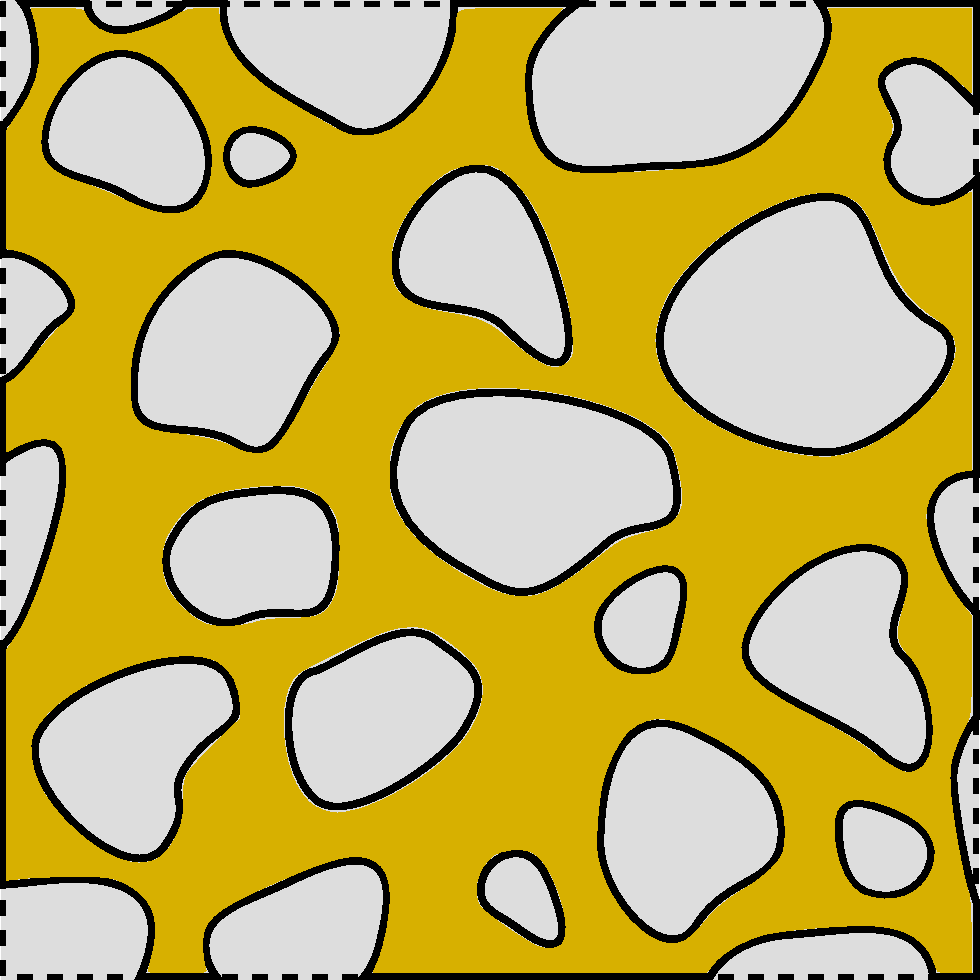
\includegraphics[scale=.3]{SwissCheeseFig}
   };
%\draw[<-, line width=.4mm] (1.6,5.0) .. controls +(up:0.5cm) and +(left:0.5cm) .. (2.5,5.7) node[right=1pt,black,text width=3cm,text badly ragged]{$\Gamma_\rve$};
\draw[<-, line width=.4mm] (5.0,3.5) .. controls +(right:0.5cm) and +(left:0.5cm) .. (6.0,3.5) node[right,black]{$\Gamma_\rve$};
\draw[<-, line width=.4mm] (4.6,2.) .. controls +(right:0.5cm) and +(left:0.5cm) .. (6.0,2.0) node[right,black]{$\Gamma_\rve^\pore$};
%\draw[-*, line width=.4mm] (-1.0,1.5) node[left=-2.0cm,black,text width=3cm,text badly ragged]{$\Omega_{\rve,i}^\mathrm{p}$} .. controls +(right:0.5cm) and +(left:1.cm) .. (0.6,1.1);
\draw[-*, line width=.4mm] (-1.0,2.1) node[left,black]{$\Omega_\rve^\particle$} .. controls +(right:0.5cm) and +(left:1.cm) .. (0.6,2.1);
\draw[-*, line width=.4mm] (-1.0,3.1) node[left,black]{$\Omega_\rve^\pore$} .. controls +(right:0.5cm) and +(left:1.cm) .. (1.2,3.1);
%\draw[<-, line width=.4mm] (4.6,1.7) .. controls +(right:0.5cm) and +(left:0.5cm) .. (6.0,1.0) node[right=1pt,black,text width=3cm,text badly ragged]{$\partial\Omega_{\rve,i}^\text{p}$};
\end{tikzpicture}
%}
\caption{Generic micro-heterogeneous material consisting of inclusions in matrix (example)}
\label{Figure1}
\end{figure}

We consider a model material as follows: The stress is decomposed in terms of deviator and pressure as $\ts{\sigma} = \ts{\sigma}_\dev - p\ts{I}$.
With the kinematic definition $\devop[\ta v]\defeq[\ta v\outerp\diff]^\sym-\frac{1}{3}[\ta v\cdot\diff]\ts{I}$, we introduce the constitutive relations
%------------------------------------------------------------------------------------------------------------
\begin{equation}
    \ts{\sigma}_\dev = \hat{\ts{\sigma}}_\dev(\devop[\ta v]), \quad
    \ta v\cdot\diff = \hat{e}(p)
\label{eq201}
\end{equation}
%------------------------------------------------------------------------------------------------------
Hence, $\hat{\ts{\sigma}}_\dev(\bullet)$ and $\hat{e}(\bullet)$ denote suitable constitutive functions.
In the simplest case of viscous fluid, we have $\hat{\ts{\sigma}}_\dev(\ts{d}_\dev)=2\mu\ts{d}_\dev$ and $\hat{e}(p)=- C p$, where $\mu(\ta{x}), C(\ta{x})$ for $\ta{x}\in\Omega$ may fluctuate strongly.
Moreover, intrinsic incompressibility is defined as $\hat{e}(p)=0$ for any value of $p$.
%------------------------------------------------------------------------------------------------------------
With micro-pores, it is also necessary to take into account surface tension, which is defined by the traction 
\begin{align}
 \ta t_\surf \defeq \gamma_\surf \hat{\ts I}\cdot\diff = -\kappa \gamma_\surf \ta n \quad\text{ on } \Gamma^\pore.
\end{align}
%------------------------------------------------------------------------------------------------------------------------
We are now in the position to formulate the strong format of the fine-scale problem under standard quasistatic conditions and small strain kinematics:
%------------------------------------------------------------------------------------------------------------
\begin{subequations}\label{eq1}
\begin{alignat}{2}
    -\left[\hat{\ts{\sigma}}_\dev(\devop[\ta v])-p\ts{I}\right]\cdot\diff & = \ta{f} &&\,\,\text{in}\,\, \Omega^\particle
 \label{eq1a} \\
    -\ta v\cdot\diff +  \hat{e}(p) & = 0 &&\,\,\text{in}\,\, \Omega^\particle
\label{eq1b} \\
    \ta v & = \ta v_\prescribed &&\,\,\text{on}\,\, \Gamma^\Dirichlet
\label{eq1c} \\
    \ta{t}\defeq\left[\hat{\ts{\sigma}}_\dev(\devop[\ta v])-p\ts{I}\right]\cdot\ta{n} & = \ta t_\prescribed &&\,\,\text{on}\,\, \Gamma^\Neumann
\label{eq1d} \\
    \ta{t}\defeq\left[\hat{\ts{\sigma}}_\dev(\devop[\ta v])-p\ts{I}\right]\cdot\ta{n} & =\ta{t}_\surf &&\,\,\text{on}\,\, \Gamma^\pore
\label{eq1surf}
\end{alignat}
\end{subequations}
%-----------------------------------------------------------------------------------------------------
The corresponding weak format is: Find $\ta v\in\set{V}, p\in\set{P}$ s.t.
%----------------------------------------------------------------------------------------------------------------
\begin{subequations}\label{eq2}
\begin{alignat}{3}
    a(\ta v;\delta\ta v) + b(p,\delta\ta v) &= l^\pore(\delta\ta v) + l(\delta\ta v) &\quad& \forall \delta\ta v &&\in \set{V}^{0}
\label{eq2a} \\
    b(\delta p,\ta v) + c^*(p;\delta p) &= 0 &\quad& \forall \delta p &&\in \set{P}
\label{eq2b}
\end{alignat}
\end{subequations}
%----------------------------------------------------------------------------------------------------------------------
where
%----------------------------------------------------------------------------------------------------------------
\begin{align}
    a(\ta{v};\ta{w}) &\defeq
    \int_{\Omega^\particle}  \devop[\ta{w}]\dprod \hat{\ts{\sigma}}_\dev(\devop[\ta{v}]) \dif V
\label{eq3a} \\
    b(q,\ta{v}) &\defeq
    - \int_{\Omega^\particle}  q\,\ta{v}\cdot\diff \dif V
\label{eq3b} \\
    c^*(q;r) &\defeq
    \int_{\Omega^\particle}  r\,\hat{e}(q) \dif V
\label{eq3c} \\
    l^\pore(\ta{v}) &\defeq -\int_{\Gamma^\pore} \gamma_\surf \hat{\ta I} \dprod [\ta{v}\outerp\diff] \dif S 
\label{eq3d} \\
    l(\ta{v}) &\defeq \int_{\Omega^\particle} \ta{v}\cdot\ta{f} \dif V + \int_{\Gamma^\Neumann} \ta{v}\cdot \ta t_\prescribed \dif S
\label{eq3e}
\end{align}
%----------------------------------------------------------------------------------------------------------------------
The solution space $\set{V}$ and the test space $\set{V}^0$ are defined in standard fashion.
In particular, all $\ta{v}\in\set{V}$ are characterized by $\ta{v}=\ta v_\prescribed$ on $\Gamma^\Dirichlet$, whereas all $\ta{v}\in\set{V}^0$ satisfy $\ta{v}=\ta{0}$ on $\Gamma^\Dirichlet$.
The pressure space $\set{P}$ does not satisfy any boundary conditions.

It is illuminating (although not necessary from an operational point of view) to invoke the potential $\Pi(\ta v,p)$
%----------------------------------------------------------------------------
\begin{align}
    \Pi(\ta v,p) &\defeq \Lambda(\ta v,p) - l^\pore(\ta v) - l(\ta v)
    \quad\mbox{with}\quad
    \Lambda(\ta v,p) \defeq \int_{\Omega} \left[\psi_\mathrm{u}(\devop[\ta v]) - p\,\ta v\cdot\diff + \psi_\mathrm{p}^*(p)\right] \dif V
\label{eq121}
\end{align}
%----------------------------------------------------------------------------
where $\psi_u(\ts{d}_\dev)$ and $\psi_p^*(p)$ are constitutive energy densities\footnote{* indicates ``complementary energy''} such that
%----------------------------------------------------------------------------
\begin{align}
    \hat{\ts{\sigma}}_\dev(\ts{d}_\dev)=\frac{\partial\psi_\mathrm{u}(\ts{d}_\dev)}{\partial\ts{d}_\dev}, &\quad
    \hat{e}(p)=\frac{\partial\psi_\mathrm{p}^*(p)}{\partial p}
\label{eq122}
\end{align}
%----------------------------------------------------------------------------
The stationarity conditions of $\Pi(\ta v,p)$ are
%----------------------------------------------------------------------------------------------------------------
\begin{subequations}\label{eq123}
\begin{alignat}{3}
    \Pi'_u(\ta v,p;\delta\ta v) &= a(\ta v;\delta\ta v) + b(p,\delta\ta v)- l^\pore(\delta\ta v)  - l(\delta\ta v) =0 &\quad& \forall \delta\ta v &&\in \set{V}^{0}
\label{eq123a} \\
    \Pi'_p(\ta v,p;\delta p) &= b(\delta p,\ta v) + c^*(p;\delta p) = 0 &\quad& \forall \delta p &&\in \set{P}
\label{eq123b}
\end{alignat}
\end{subequations}
%----------------------------------------------------------------------------------------------------------------------
which are identical to the weak form in \cref{eq2}.

Here we highlight the differences from weak format in the previous work [paper3]:
\begin{itemize}
\item The sub-scale domain is only $\Omega^\particle \subseteq \Omega$.
\item The surface-tension load $l^\pore(\ta v)$ in \eqref{eq2a}
\end{itemize}
In the special case that $\Omega^\particle = \Omega$, and thus $\Gamma^\pore = \emptyset$, then we retain exactly the same problem as in [paper3].

\section{Variationally Consistent Homogenization}

\subsection{VMS-ansatz and scale separation}

The appropriate variational setting of the homogenized problem is obtained upon replacing the integrands in the weak forms in \crefrange{eq3a}{eq3d} by running averages of the type
%----------------------------------------------------------------------------
\begin{align}
    y \mapsto
    \homgen{y} &\defeq \frac{1}{\volume}\int_{\Omega_\rve^\particle} y \dif V, \quad \Omega_\rve^\particle = \Omega^\particle \cap\Omega_\rve
    \label{eq16a}
\intertext{and for the internal surface $\Gamma^\pore$}
    y \mapsto
    \shomgen{ y } &\defeq \frac{1}{\volume}\int_{\Gamma_\rve^\pore} y \dif S, \quad \Gamma_\rve^\pore = \Gamma^\pore \cap\Omega_\rve
    \label{eq16b}
\end{align}
%----------------------------------------------------------------------------
representing a smoothing approximation on a RVE.
In practice, the RVE's are finite-sized and occupies the subscale region $\Omega_\rve$ with boundary $\Gamma_\rve$.
The typical dimension of an RVE is $L_\rve=\volume^{1/3}$.
The RVE is centered at the macroscale position $\bar{\ta{x}}\defeq\frac{1}{|\Gamma_\rve|}\int_{\Gamma_\rve} \ta{x}\dif S$ for any given $\bar{\ta{x}}\in\Omega$.
Boundary integrals can be homogenized in similar fashion, by considering Representative Surface Elements $\Gamma_\#$
\begin{align}
 y \to \langle y \rangle_{\#} \defeq \frac{1}{|\Gamma_\#|} \int_{\Gamma_\#} y \dif S
\end{align}


The weak forms in \crefrange{eq3a}{eq3e} are thus approximated as
%----------------------------------------------------------------------------------------------------------------
\begin{align}
    a(\ta{v};\ta{w}) &\approx \int_\Omega a_\rve(\ta{v};\ta{w}) \dif V
\label{eq7a} \\
    b(q,\ta{v}) &\approx \int_\Omega b_\rve(q,\ta{v}) \dif V
\label{eq7b} \\
    c^*(q;r) &\approx \int_\Omega c^*_\rve(q;r) \dif V
\label{eq7c} \\
    l(\ta{v}) &\approx \int_\Omega l_\rve(\ta{v}) \dif V + \int_{\Gamma^\Neumann} l_\#(\ta{v}) \dif S
\label{eq7d} \\
    l^\pore(\ta{v}) &\approx \int_\Omega l_\rve^\pore(\ta v) \dif V
\label{eq7e}
\end{align}
%---------------------------------------------------------------------------------------------------------------------
where the RVE-functionals in \crefrange{eq7a}{eq7d} are defined as
%----------------------------------------------------------------------------------------------------------------
\begin{align}
    a_\rve(\ta{v};\ta{w}) &\defeq
    \homgen{ \devop[\ta{w}]\dprod \hat{\ts{\sigma}}_\dev(\devop[\ta{v}]) }
\label{eq8a} \\
    b_\rve(q,\ta{v}) &\defeq
    -  \homgen{ q\,\ta{v}\cdot\diff }
\label{eq8b} \\
    c^*_\rve(q;r) &\defeq
    \homgen{ r\,\hat{e}(q) }
\label{eq8c} \\
    l_\rve^\pore(\ta{v}) &\defeq
    \shomgen{ \gamma_\surf \hat{\ts I} \dprod [\ta{v}\outerp\diff] }
\label{eq8d} \\
    l_\rve(\ta{v}) &\defeq
    \homgen{ \ta{v}\cdot\ta{f} }, \quad
    l_\#(\ta{v}) \defeq
    \langle \ta{v}\cdot \ta t_\prescribed \rangle_\#
\label{eq8e}
\end{align}
%---------------------------------------------------------------------------------------------------------------------
Likewise, we homogenize the volume-specific energy potential $\Lambda(\ta v,p)$:
%----------------------------------------------------------------------------
\begin{align}
    \Lambda(\ta{v},q) &\approx \int_\Omega \Lambda_\rve(\ta{v},q) \dif V
\label{eq222}
\end{align}
%----------------------------------------------------------------------------
where the RVE-functional $\Lambda_\rve(\ta{v},q)$ is given as
%----------------------------------------------------------------------------
\begin{align}
    \Lambda_\rve(\ta{v},q) &\defeq
    \homgen{ \psi_u(\devop[\ta{v}])}
    + l_\rve^\pore(\ta{v}) 
    - \homgen{  p\,\ta{v}\cdot\diff } + \homgen{ \psi_p^*(q) }
\label{eqRveBulkPotential}
\end{align}
%----------------------------------------------------------------------------
Note in particular the treatment of the surface tension in \eqref{eq7e}, which exists now only in the RVE-problem, and influences the macroscale problem only through \eqref{eq7a} and \eqref{eq7b}.

In the spirit of the Variational MultiScale method (VMS) \cite{larsson_variationally_2010}, we introduce the \emph{ansatz} that the fields $\ta v\in\set{V}$ and $p\in\set{P}$ can be decomposed into macroscale (smooth) and subscale (fluctuating) parts inside each RVE via the unique orthogonal split $\set{V} = \set{V}^\macro \oplus \set{V}^\fluct$ and $\set{P} = \set{P}^\macro \oplus \set{P}^\fluct$.
As a result, we may assume that it is possible solve for the fluctuation fields $\ta v^\fluct\in\set{V}^\fluct$ and $p^\fluct\in\set{P}^\fluct$ as ``local approximations'' on each RVE for given macroscale solutions $\ta v^\macro\in\set{V}^\macro$ and $p^\macro\in\set{P}^\macro$, i.e.\ we construct the complete solution on each RVE as\footnote{Curly brackets $\{(\bullet)\}$ indicate implicit and/or nonlocal functional dependence on $(\bullet)$.}.
%------------------------------------------------------------------------------------------------------------
\begin{subequations}\label{eq4}
\begin{alignat}{2}
    \ta v\approx \tilde{\ta v}\{\ta v^\macro,p^\macro\} &\defeq \ta v^\macro+\tilde{\ta v}^\fluct\{\ta v^\macro,p^\macro\} &&\text{ in } \Omega_\rve
\label{eq4a} \\
    p\approx \tilde{p}\{\ta v^\macro,p^\macro\} &\defeq p^\macro+\tilde{p}^\fluct\{\ta v^\macro,p^\macro\} &&\text{ in } \Omega_\rve
\label{eq4b}
\end{alignat}
\end{subequations}
%------------------------------------------------------------------------------------------------------------
On the boundary of the macroscale domain, $\Gamma$, we assume smooth variation of $\ta v$ defined by the explicit relations $\ta v = \ta v^\macro$, $p = p^\macro$ on $\Gamma_\#$.


In addition, the test function $\delta\ta v\in\set{V}^{0}$ in \cref{eq2a} is replaced by $\delta\ta v^\macro\in\set{V}^{\macro,0}$, whereas $\delta p\in\set{P}$ in \cref{eq2b} is replaced by $\delta p^\macro\in\set{P}^{\macro}$.
Altogether, these assumptions infer that $\ta v^\macro\in\set{V}^\macro$ and $p^\macro\in\set{P}^\macro$ can be solved from the homogenized problem
%----------------------------------------------------------------------------------------------------------------
\begin{subequations}\label{eq6}
\begin{alignat}{3}
    a(\tilde{\ta v}\{\ta v^\macro,p^\macro\};\delta\ta v^\macro) +
    b(\tilde{p}\{\ta v^\macro,p^\macro\},\delta\ta v^\macro)
    &= l(\delta\ta v^\macro)
    &\quad& \forall \delta\ta v^\macro &&\in \set{V}^{\macro,0}
\label{eq6a} \\
    b(\delta p^\macro,\tilde{\ta v}\{\ta v^\macro,p^\macro\}) +
    c^*(\tilde{p}\{\ta v^\macro,p^\macro\};\delta p^\macro)
    &= 0 &\quad& \forall \delta p^\macro &&\in \set{P}^{\macro}
\label{eq6b}
\end{alignat}
\end{subequations}
%----------------------------------------------------------------------------------------------------------------------

\subsection{Explicit format of macroscale (homogenized) problem}
In practice, the scales are linked  by expressing $\ta v^\macro(\bar{\ta{x}},{\ta{x}})$\footnote{Double arguments, i.e.\ $\ta v(\bar{\ta{x}},\ta{x})$, are used to explicitly point out the underlying scale separation.} and $p^\macro(\bar{\ta x},\ta x)$ using Taylor series expansions of suitable order for $\bar{\ta{x}}\in\Omega$ and $\ta{x}\in\Omega_\rve(\bar{\ta{x}})$
in terms of the macroscale solution $\bar{\ta v}(\bar{\ta{x}})$ and $\bar{p}(\bar{\ta x})$ respectively. However, in this case we must take into account both porosity and surface tension in order to obtain the simplest macroscale format.
We thus introduce the macroscale fields $(\bar{\ta v},\bar{p})\in\bar{\set{V}}\times\bar{\set{P}}$ such that the macroscale solutions $\ta v^\macro, p^\macro$ inside each RVE are expanded as follows:
%----------------------------------------------------------------------------
\begin{subequations}\label{eq12}
\begin{align}
    \ta v^\macro(\bar{\ta{x}};\ta{x}) &= \bar{\ta v}(\bar{\ta{x}}) + \bar{\ts{h}}(\bar{\ta{x}}) \cdot [\ta{x}-\bar{\ta{x}}], \quad \bar{\ts{h}}\defeq\bar{\ta v}\outerp\diff, \quad \ta{x}\in\Omega_\rve
\label{eq12a} \\
    p^\macro(\bar{\ta{x}};\ta{x}) &= \densinv [\bar{p}(\bar{\ta{x}}) + \frac23 \shomgen{\gamma_\surf}], \quad
    \ta{x}\in\Omega_\rve
\label{eq12b}
\end{align}
\end{subequations}
%----------------------------------------------------------------------------
Hence, $\ta v^\macro$ is assumed to have linear variation in $\Omega_\rve$ pertinent to standard ``first order homogenization'', whereas $p^\macro$ is constant in $\Omega_\rve$.
We have also introduced the inverse of the relative density, defined as $\densinv \defeq \frac{\volume}{|\Omega_\rve^\particle|}$.
Now, we require that
%----------------------------------------------------------------------------
\begin{subequations}\label{eq14}
\begin{gather}
    \frac{1}{|\Gamma_\rve|} \int_{\Gamma_\rve} \ta v \dif S = \bar{\ta v}, \quad
    \frac{1}{\volume} \int_{\Gamma_\rve} \ta v \outerp \ta n \dif S = \bar{\ta{h}}
\label{eq14a} \\
    %\frac{1}{\volume} \int_{\Gamma_\rve} p\,\ta n \cdot [\ta x-\bar{\ta x}] \dif S = \bar{p}
    \homgen{p} - \frac23 \shomgen{\gamma_\surf} = \bar{p}
\label{eq14b}
\end{gather}
\end{subequations}
which leads to the constraints
%----------------------------------------------------------------------------
\begin{subequations}\label{eq13}
\begin{gather}
    \frac{1}{|\Gamma_\rve|} \int_{\Gamma_\rve} \ta v^\fluct \dif S = \ta 0, \quad
    \frac{1}{\volume} \int_{\Gamma_\rve} \ta v^\fluct \outerp \ta n \dif S = \ts 0
\label{eq13a} \\
    \homgen{p^\fluct} = 0
\label{eq13b}
\end{gather}
\end{subequations}
%----------------------------------------------------------------------------
As a result, the hierarchical split ($\set{V} = \set{V}^\macro \oplus \set{V}^\fluct$ and $\set{P} = \set{P}^\macro \oplus \set{P}^\fluct$) is guaranteed.
%----------------------------------------------------------------------------
We can thus establish at the outset, before any further analysis, that the velocity and pressure fields within each RVE are implicit functions of the values $\bar{\ta v}$, $\bar{\ts h}$, $\bar{p}$, such that $\ta v = \tilde{\ta v}\{\bar{\ta v}, \bar{\ts h}, \bar{p}\}$ and $p = \tilde{p}\{\bar{\ta v}, \bar{\ts h}, \bar{p}\}$.

With the representations in \cref{eq12} and the constraints in \cref{eq14,eq13}, we are in the position to compute the homogenized quantities that enter the system \cref{eq6}:
%----------------------------------------------------------------------------------------------------------------
%\todo{$\delta u^\macro$ in RHS but not in LHS}
\begin{align}
    a_\rve(\ta v;\delta\ta v^\macro) &=
    \homgen{ \hat{\ts{\sigma}}_\dev(\devop[\ta v]) } \dprod \devop[\delta\bar{\ta v}] 
\label{eq15a} \\
    b_\rve(p,\delta\ta v^\macro) &=
    -  \homgen{ p }\, \delta\bar{\ta v}\cdot\diff
\label{eq15b} \\
    b_\rve(\delta p^\macro,\ta v) &=
    - \densinv\delta\bar{p}\, \homgen{ \ta v\cdot\diff } = - \delta\bar{p} \, \bar{\ta v}\cdot\diff - \densinv\delta\bar{p}\,\homgen{ \ta v^\fluct\cdot\diff }
\label{eq15c} \\
    c^*_\rve(p;\delta p^\macro) &=
    \densinv\delta\bar{p}\, \homgen{ \hat{e}(p) }
\label{eq15d} \\
    l_\rve^\pore(\delta\ta v^\macro) &=
    -\shomgen{ \gamma_\surf \hat{\ts I} } \dprod [\delta\bar{\ta v}\outerp\diff]
\label{eq15e} \\
    l_\rve(\delta\ta v^\macro) &=
    \delta\bar{\ta v}\cdot \bar{\ta f} + [\delta\bar{\ta v}\outerp\diff]\dprod \bar{\bar{\ta f}}
\label{eq15f} \\
    l_\#(\delta\ta v^\macro) &=
    \delta\bar{\ta v} \cdot \bar{\ta t}_\prescribed + [\delta\bar{\ta v}\outerp\diff]\dprod \bar{\bar{\ta{t}}}_\prescribed
\label{eq15g}
\end{align}
%---------------------------------------------------------------------------------------------------------------------
The applied macroscale loads $\bar{\ta f}$, $\bar{\ta t}_\prescribed$ and ``moments'' $\bar{\bar{\ta f}}$, $\bar{\bar{\ta t}}_\prescribed$ are defined as
%----------------------------------------------------------------------------------------------------------------
\begin{alignat}{2}
    \bar{\ta f} &= \homgen{ \ta{f} },\quad
    &\bar{\bar{\ta f}} &= \homgen{ \ta{f}\outerp[\ta{x}-\bar{\ta{x}}] }
\label{eq15fa}
\\
    \bar{\ta t}_\prescribed &= \langle \ta{t}_\prescribed \rangle_\#,\quad
    &\bar{\bar{\ta t}}_\prescribed &= \langle \ta{t}_\prescribed\outerp[\ta{x}-\bar{\ta{x}}]  \rangle_\#
\end{alignat}
%---------------------------------------------------------------------------------------------------------------------
\textbf{Remark:} Henceforth, we restrict to the situation when $\volume\to 0$ and $|\Gamma_\#|\to 0$; hence $\bar{\bar{\ta f}}$ and $\bar{\bar{\ta t}}_\prescribed$ will vanish.
We will also consider $\bar{\ta f}$ and $\bar{\ta t}_\prescribed$ as given macroscopic quantities. $\Box$

Plugging \cref{eq15a,eq15b,eq15c,eq15d,eq15e,eq15f,eq15g} into \cref{eq6} weak form we get
\begin{subequations}\label{eq:derived_macro}
\begin{align}
 \int_\Omega \underbrace{[\homgen{ \hat{\ts{\sigma}}_\dev(\devop[\ta v]) - p \ts I } + \shomgen{ \gamma_\surf \hat{\ts I}}]}_{=\bar{\ts\sigma}_\dev - \bar{p}\ts I} \dprod [\delta\bar{\ta v}\outerp\diff] \dif V &= 
  \int_\Omega \bar{\ta f} \cdot \delta\bar{\ta v} \dif V + 
  \int_\Gamma \bar{\ta t}_\prescribed \cdot \delta\bar{\ta v} \dif S
\label{eq:derived_macro_a}
\\
 \int_\Omega \Big[ - \delta\bar{p}\, \bar{\ta v}\cdot\diff + \delta\bar{p}\, \underbrace{\densinv\homgen{ \hat{e}(p) - \ta v^\fluct\cdot\ta n}}_{\bar{e}} \Big]\dif V &= 0
\label{eq:derived_macro_b}
\end{align}
\end{subequations}
where we continue to manipulate \cref{eq:derived_macro_a} further
\begin{align}
 \homgen{ \hat{\ts{\sigma}}_\dev(\devop[\ta v]) - p \ts I } + \shomgen{ \gamma_\surf \hat{\ts I}}
  = \homgen{ \ts{\sigma} } + \shomgen{ \gamma_\surf \hat{\ts I}}
\nonumber\\
  = \frac{1}{\volume} \Big[ \int_{\Gamma_\rve \cup \Gamma_\rve^\pore } \ta t \outerp[\ta x-\bar{\ta x}] \dif S + \shomgen{ \gamma_\surf \hat{\ts I}} \Big]
\nonumber\\
  = \frac{1}{\volume} \Big[\int_{\Gamma_\rve} \ta t \outerp[\ta x-\bar{\ta x}] \dif S + \int_{\Gamma_\rve^\pore } [\ta t_\surf \outerp[\ta x-\bar{\ta x}] + \gamma_\surf \hat{\ts I} ]\dif S \Big]
\nonumber\\
  = \frac{1}{\volume} \Big[\int_{\Gamma_\rve} \ta t \outerp[\ta x-\bar{\ta x}] \dif S + \int_{\partial\Gamma_\rve^\pore} \hat{\ta t}\outerp[\ta x - \bar{\ta x}]\dif C \Big]
 \label{eq:derived_macro_a2}
\end{align}
Since pore boundaries on $\Gamma_\rve$ is not applicable for the weakly periodic or Neumann boundary condition, we henceforth limit the RVE's to have no pores crossing the boundary $\Gamma_\rve$, and as such the integral over $\partial\Gamma_\rve^\pore$ also vanishes. Thus we are in position to define the macroscopic deviatoric stress and volumetric strain
%----------------------------------------------------------------------------------------------------------------
\begin{align}
    \bar{\ts{\sigma}}_\dev \defeq \frac{1}{\volume}\int_{\Gamma_\rve} \ta t \outerp[\ta x-\bar{\ta x}] \dif S + \bar{p}\ts I, \, \quad
    \bar{e} \defeq \densinv\homgen{ \hat{e}(p) - \ta v^\fluct\cdot\diff}
\label{eq16}
\end{align}
%----------------------------------------------------------------------------------------------------------------
We note that $\bar{\ts\sigma}_\dev$ and $\bar{e}$ are indeed implicit functions of the values of the macroscale variables $\bar{\ta v}$, $\bar{\ts h}$ and $\bar{p}$, pertinent to the considered RVE.

\noindent\textbf{Remark:} If one wants to include a non-empty $\partial\Gamma_\rve^\pore$, then \cref{eq14b} also needs to include the corresponding term in order obtain the same macroscopic problem. $\Box$

Finally, we may express the macroscale problem the abstract form:
Find $(\bar{\ta v},\bar{p})\in\bar{\set{V}}\times\bar{\set{P}}$ that solve
%----------------------------------------------------------------------------------------------------------------
\begin{subequations}\label{eq:macro}
\begin{alignat}{3}
    \bar{a}(\bar{\ta v},\bar{p};\delta\bar{\ta v}) + \bar{b}(\bar{p},\delta\bar{\ta v}) &= \bar{l}(\delta\bar{\ta v})
      &\quad& \forall \delta\bar{\ta v} &&\in \bar{\set{V}}^{0}
\label{eq:macro_a} \\
    \bar{b}(\delta\bar{p},\bar{\ta v}) + \bar{c}^*(\bar{\ta v},\bar{p};\delta\bar{p}) &= 0
      &\quad& \forall \delta\bar{p} &&\in \bar{\set{P}}
\label{eq:macro_b}
\end{alignat}
\end{subequations}
%----------------------------------------------------------------------------------------------------------------------
where
%----------------------------------------------------------------------------------------------------------------
\begin{align}
    \bar{a}(\bar{\ta v},\bar{p};\bar{\ta w}) &\defeq
    \int_{\Omega}  \devop[\bar{\ta w}]\dprod\bar{\ts\sigma}_\dev\{\bar{\ta v}, \bar{p}\} \dif V
\label{eq18a} \\
    \bar{b}(\bar{q},\bar{\ta v}) &\defeq
    - \int_{\Omega}  \bar{q}\,\bar{\ta v}\cdot\diff \dif V
\label{eq18b} \\
    \bar{c}^*(\bar{\ta v},\bar{p};\bar{r}) &\defeq
    \int_{\Omega}  \bar{r}\,\bar{e}\{\bar{\ta v}, \bar{p}\} \dif V
\label{eq18c} \\
    \bar{l}(\bar{\ta v}) &\defeq  \int_{\Omega}  \bar{\ta v}\cdot\bar{\ta f} \dif V +
    \int_{\Gamma^\Neumann} \bar{\ta v}\cdot\bar{\ta t}_\prescribed \dif S
\label{eq18d}
\end{align}
%----------------------------------------------------------------------------------------------------------------------
If we consider the macroscale fields, $\bar{\ts\sigma}_\dev$ and $\bar{e}$,  we conclude that they are implicit functions of the fields $\bar{\ta v}$ and $\bar{p}$.
The macroscale spaces $\bar{\set{V}}$ and $\bar{\set{P}}$ are chosen as the standard ones for the fine-scale problem.

We remark that we have obtained the same macroscale problem as in [paper3].
The only difference is how the response variables, $\bar{\ts\sigma}_\dev$ and $\bar{e}$ are identified.
In order to obtain the desired format in \eqref{eq:macro}, we have to carefully define $p^\macro$ in \eqref{eq12b} to incorporate the volumetric part of the surface tension as well as the volume ratio. However, this particular definition leads to a very simple constraint for the fluctuation $p^\fluct$ in \eqref{eq13b} which will prove useful for the RVE-problem.
In the special case $\Omega^\particle = \Omega$, we again retain the same expression for $\bar{e}$ and $\bar{\ts\sigma}_\dev$ as in [paper3].



\section{Canonical formulation of RVE-problem}

\subsection{Preliminaries -- Concept of weak periodicity of fluctuation velocity}

We will now propose an RVE problem in the same manner as in [paper3], with the modifications that the domain is $\Omega^\particle$ and the inclusion of the surface tension load:
%----------------------------------------------------------------------------
\begin{subequations}
\begin{align}
    a_\rve(\ta v;\delta\ta v) + b_\rve(\delta\ta v,p) - \frac{1}{\volume}\int_{\Gamma_\rve} \ta{t}\cdot\delta\ta v \dif S &= l_\rve^\pore(\delta\ta v)
\label{eq19a} \\
    b_\rve(\ta v,\delta p) + c^*_\rve(p;\delta p) &= 0
\label{eq19b}
\end{align}
\end{subequations}
\todo{skip a lot?}
%---------------------------------------------------------------------------
which is supposed to hold true for all possible $\delta\ta v, \delta p$ in suitable function spaces (as discussed below).
However, this problem is not solvable without further specification of the solution fields $\ta v, p, \ta{t}$.
In this paper we adopt a recently proposed variational framework allowing for \emph{weak satisfaction of micro-periodicity}, cf.\  Larsson et al.\ \cite{larsson_computational_2011}, and this framework will be briefly summarized in what follows.
We then \emph{assume} that the subscale fluctuation field $\ta v^\fluct$ is periodic across the RVE boundaries w.r.t.\ the chosen local coordinate axes.
This model assumption, which may be termed ``micro-periodicity'', is a key ingredient (and frequently adopted) in the literature on mathematical homogenization and can be viewed as an approximation between the stiffer Dirichlet and the weaker Neumann boundary conditions.
Indeed, both these cases can be obtained as special cases of the most general variational format of periodicity (as will be discussed further below).

In order to formulate the conditions on micro-periodicity, we consider the RVE in \cref{Figure2}, where the boundary $\Gamma_\rve$ has been split into two parts: $\Gamma_\rve=\Gamma_\rve^- \cup \Gamma_\rve^+$.
Here, $\Gamma_\rve^+$ is the \emph{image boundary} (later chosen as the computational domain for boundary integration), whereas $\Gamma^-$ is the \emph{mirror boundary}.
We shall now introduce the proper mapping $\ta{\varphi}_\per:\Gamma^+ \rightarrow \Gamma^-$ such that any point $\ta{x}^+\in\Gamma_\rve^+$ is mirrored in a self-similar fashion to the corresponding point $\ta{x}^-\in\Gamma_\rve^-$; hence, $\ta{x}^-=\ta{\varphi}_\per(\ta{x}^+)$.
%---------------------------------------------------------------------------------
\begin{figure}[H]
\centering
\begin{tikzpicture}
%\tikzstyle{every node}=[font=\Large]
\node [inner sep=0pt,above right]{
   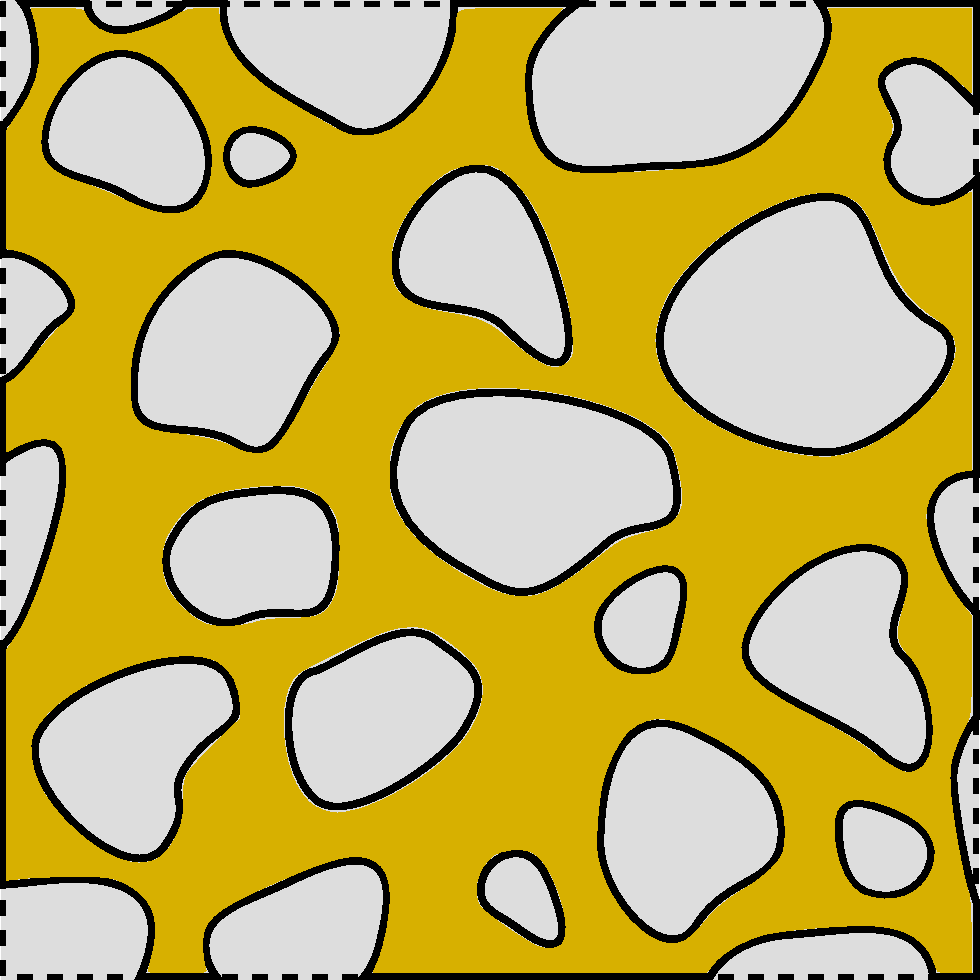
\includegraphics[scale=.3]{SwissCheeseFig}
   };
\draw[<-, line width=.4mm] (5.0,4.0) to[out=0,in=-120] (6.0,5.0) node[right=1pt,black]{$\Gamma_\rve^+$};
\draw[<-, line width=.4mm] (4.0,5.0) to[out=60,in=120] (6.0,5.0);
\draw[<-, line width=.4mm] (0.0,1.0) to[out=180,in=60] (-1.0,0.0) node[left=1pt,black]{$\Gamma_\rve^-$};
\draw[<-, line width=.4mm] (1.0,0.0) to[out=-120,in=-60] (-1.0,0.0);
\draw[<-, line width=.6mm] (0.0,2.4) to[out=15,in=165] (5.0,2.4) node[right]{$\ta{\varphi}_\per$} ;
%\draw[<-, line width=.4mm] (4.6,1.7) .. controls +(right:0.5cm) and +(left:0.5cm) .. (6.0,1.0) node[right=1pt,black,text width=3cm,text badly ragged]{$\partial\Omega_{\rve,i}^\text{p}$};
\end{tikzpicture}
\caption{RVE in 2D with ``image'' and ``mirror'' boundaries.}
\label{Figure2}
\end{figure}
%--------------------------------------------------------------------------------
In particular, we express micro-periodicity of the velocity fluctuation field as
%--------------------------------------------------------------------------------
\begin{equation}
    \ta v^\fluct(\ta{x}) = \ta v^\fluct(\ta{\varphi}_\per(\ta{x})), \quad
    \forall \ta{x}\in\Gamma_\rve^+
\label{eq21}
\end{equation}
%---------------------------------------------------------------------------
or, equivalently, in terms of the ``jump'' between the fluctuation fields on the image and mirror parts of the boundary as follows:
%--------------------------------------------------------------------------------
\begin{equation}
    \jmp{\ta v^\fluct} = \ta{0} \quad \makebox{on } \Gamma_\rve^+, \quad
    \jmp{\ta v^\fluct}(\ta{x}) \defeq \ta v^\fluct(\ta{x})-\ta v^\fluct(\ta{\varphi}_\per(\ta{x}))
\label{eq22}
\end{equation}
%---------------------------------------------------------------------------

Subsequently, we shall not enforce the condition \cref{eq22} strongly as the point of departure; rather it is done weakly.
To this end, we first assume that $\ts{\sigma}$ satisfies the \emph{symmetry condition}
%--------------------------------------------------------------------------------
\begin{equation}
    \ts{\sigma}(\ta{x}) = \ts{\sigma}(\ta{\varphi}_\per(\ta{x})), \quad
    \forall \ta{x}\in\Gamma_\rve^+
\label{eq23}
\end{equation}
%---------------------------------------------------------------------------
As an immediate consequence of this symmetry assumption, we obtain that the boundary tractions $\ta{t}\defeq\ts{\sigma}\cdot\ta{n}$ satisfy the following \emph{anti-symmetry condition} for any mirror point (that is not a corner point)
%--------------------------------------------------------------------------------
\begin{equation}
    \ta{t}(\ta{x}) = -\ta{t}(\ta{\varphi}_\per(\ta{x})), \quad
    \forall \ta{x}\in\Gamma_\rve^+
\label{eq24}
\end{equation}
%---------------------------------------------------------------------------
as depicted in \cref{Figure2}.
We now evaluate, upon using \cref{eq24}, the boundary term in
\cref{eq19a}, as follows:
%----------------------------------------------------------------------------
\begin{equation}
    \int_{\Gamma_\rve} \ta{t} \cdot \delta \ta v \dif S =
    \int_{\Gamma_\rve^+} \ta{t} \cdot \jmp{\delta \ta v} \dif S
\label{eq25}
\end{equation}
%----------------------------------------------------------------------------

A weak statement of the micro-periodicity constraint, given in strong form in \cref{eq23}, is
%--------------------------------------------------------------------------------
\begin{equation}
    \frac{1}{\volume}\int_{\Gamma_\rve^+} \delta \ta{t} \cdot \jmp{\ta v^\fluct} \dif S = 0,
    \quad \forall \delta \ta{t}\in\set{T}_\rve
\label{eq26}
\end{equation}
%---------------------------------------------------------------------------
where the space of test functions that ``live'' only on the image boundary $\Gamma_\rve^+$ is given as:
%----------------------------------------------------------------------------
\begin{equation}
    \set{T}_\rve = [L_2(\Gamma_\rve^+)]^{3}
\label{eq25a}
\end{equation}
%----------------------------------------------------------------------------
Associated with this condition, we introduce the auxiliary variational form
%----------------------------------------------------------------------------
\begin{equation}
    d_\rve(\ta{t},\ta v) \defeq
    - \frac{1}{\volume}\int_{\Gamma_\rve^+} \ta{t} \cdot \jmp{\ta v} \dif S
\label{eq27}
\end{equation}
%----------------------------------------------------------------------------
whereby the constraint \cref{eq26} is expressed as
%----------------------------------------------------------------------------
\begin{equation}
    d_\rve(\delta\ta{t},\ta v^\fluct) = 0, \quad \forall \delta \ta{t}\in\set{T}_\rve
\label{eq27a}
\end{equation}
%----------------------------------------------------------------------------

\subsection{RVE-problem -- Original ``variationally consistent'' weak format}
\label{sec:original_rve}

In order to establish the most straightforward formulation of the RVE-problem, based on micro-periodicity, we first use the constraints in \cref{eq13} and introduce the following spaces for the fluctuation fields:
%----------------------------------------------------------------------------
\begin{align}
    \set{V}_\rve^\fluct &= \{\ta{v}\in [H^1(\Omega_\rve)]^{3} \,| \quad \frac{1}{|\Gamma_\rve|}\int_{\Gamma_\rve} \ta{v} \dif S = \ta 0, \quad
    \frac{1}{\volume} \int_{\Gamma_\rve} \ta v^\fluct \outerp \ta n \dif V = \ts 0 \}
\label{eq28a} \\
    \set{P}_\rve^\fluct &= \{q\in L_2(\Omega_\rve) \,| \quad \homgen{q} = 0 \}
\label{eq28b}
\end{align}

It is then obvious that, for given macroscale values $\bar{\ta v}$, $\bar{\ts h}$, and $\bar{p}$, we can introduce the unique decompositions
\begin{subequations}\label{eq29}
\begin{alignat}{2}
    \ta v &= \bar{\ta v} + \bar{\ts{h}} \cdot [\ta{x}-\bar{\ta{x}}] + \ta v^\fluct, &\quad& \ta v^\fluct\in\set{V}_\rve^\fluct
\label{eq29a} \\
     p     &= \densinv [\bar{p} + \frac23 \shomgen{\gamma_\surf}] + p^\fluct, &\quad& p^\fluct\in\set{P}_\rve^\fluct
\label{eq29b}
\end{alignat}
\end{subequations}
Next, we aim for a unique decomposition of the tractions (which are anti-periodic by assumption) in a fashion that is similar to \cref{eq29}.
To this end, we first associate each traction field $\ta t$ along $\Gamma_\rve$ with the average stress $\bar{\ts\tau}[\ta t] \in \set{R}^{3\times 3}$, defined as
\begin{align}
 \bar{\ts\tau}[\ta t] = \frac{1}{\volume} \int_{\Gamma_\rve^+} \ta t \outerp \jmp{\ta x - \bar{\ta x}} \dif S
\label{eq:t_average}
\end{align}
This definition for the average stress is chosen so that for any stress field $\ts\tau$ in equilibrium and such that $\ta t = \ts\tau\cdot\ta n$ on $\Gamma_\rve^+$  we obtain 
$\bar{\ts\tau} = \frac{1}{\volume}\int_{\Gamma_\rve} \ts\tau\cdot\ta n \outerp \jmp{\ta x - \bar{\ta x}}\dif S$.
We also conclude that 
\begin{align}
d_\rve(\bar{\ts\tau}\cdot \ta n, \ta v^\fluct) = 0\quad \forall\ta v^\fluct\in\set{V}_\rve^\fluct,\;\bar{\ts\tau}\in\set{R}^{3\times3}.
\label{eq:dtauu0}
\end{align}
As a direct consequence of \cref{eq:t_average}, we may introduce the unique split
\begin{align}
 \ta t = \bar{\ts\tau}\cdot\ta n + \ta t^\fluct,\quad \bar{\ts\tau}\in \set{R}^{3\times3},\;\ta t^\fluct\in \set{T}_\rve^\fluct
\label{eq:t_split}
\end{align}
where $\set{T}_\rve^\fluct$ is the space of the traction fluctuations that are self-equilibrating and thus defined as
\begin{align}
 \set{T}_\rve^\fluct &= \{\ta{s}\in [L_2(\Gamma_\rve^+)]^{3} \,| \quad \bar{\ts\tau}[\ta s] = \frac{1}{\volume}\int_{\Gamma_\rve^+} \ta{s}\outerp\jmp{\ta{x}-\bar{\ta{x}}} \dif S = \ta{0} \}
 \label{eq28c}
\end{align}
% C2:
The proof of uniqueness of the split in \cref{eq:t_split} follows from the identity
\begin{align}
\ta t = \bar{\ts\tau}[\ta t]\cdot\ta n + [\ta t - \bar{\ts\tau}[\ta t]\cdot\ta n]
\end{align}
and the fact that
\begin{align}
 \bar{\ts\tau}[\ta t - \bar{\ts\tau}[\ta t]\cdot\ta n] = \bar{\ts\tau}[\ta t] - \bar{\ts\tau}[\bar{\ts\tau}[\ta t]\cdot\ta n] = \bar{\ts\tau}[\ta t] - \bar{\ts\tau}[\ta t] = 0
\end{align}
Hence, $\ta t^\fluct \defeq \ta t - \bar{\ts\tau}[\ta t]\cdot\ta n \in\set{T}_\rve^\fluct$. $\Box$

As preliminaries for establishing the RVE-problem, we establish two identities:
Firstly, from \cref{eq:dtauu0,eq:t_split} follows that
\begin{align}
d_\rve(\ta t,\delta\ta v^\fluct) = d_\rve(\ta t^\fluct, \delta\ta v^\fluct)\quad \forall\delta\ta v^\fluct \in\set{V}_\rve^\fluct
\end{align}
Secondly, it follows from \cref{eq12a} and the properties of $\set{P}_\rve^\fluct$ that
\begin{equation}
    b_\rve(\delta p^\fluct,\ta v) = b_\rve(\delta p^\fluct,\ta v^\fluct) \quad\forall \delta p^\fluct\in\set{P}_\rve^\fluct
\label{eq27c}
\end{equation}
whereby it is noted that the macroscale part of $\ta v$ is ``filtered out''.



We are now in the position to establish the subscale problem:
For \emph{given} values $\bar{\ta v}$, $\bar{\ts{h}}$, and $\bar{p}$, that represent the macroscale fields (and which solve the macroscale problem), find the subscale fluctuations $(\ta v^\fluct,p^\fluct,\ta{t}^\fluct)\in\set{V}_\rve^\fluct\times\set{P}_\rve^\fluct\times\set{T}_\rve^\fluct$ that solve the system
%----------------------------------------------------------------------------
\begin{subequations}\label{eq31}
\begin{alignat}{3}
    a_\rve(\bar{\ts d}_\dev\cdot [\ta{x}-\bar{\ta{x}}]+\ta v^\fluct;\delta\ta v^\fluct) +
    b_\rve(\densinv [\bar{p} + \frac23 \shomgen{\gamma_\surf}] +p^\fluct,\delta\ta v^\fluct) +
    d_\rve(\ta{t}^\fluct,\delta\ta v^\fluct) &= l_\rve^\pore(\delta\ta v^\fluct)
    &\quad& \forall \delta\ta v^\fluct &&\in \set{V}_\rve^\fluct
\label{eq31a} \\
    b_\rve(\delta p^\fluct,\ta v^\fluct) + c^*_\rve(\densinv [\bar{p} + \frac23 \shomgen{\gamma_\surf}] +p^\fluct;\delta p^\fluct) &= 0
    &\quad& \forall \delta p^\fluct &&\in \set{P}_\rve^\fluct
\label{eq31b} \\
    d_\rve(\delta\ta{t}^\fluct,\ta v^\fluct) &= 0
    &\quad& \forall \delta \ta{t}^\fluct &&\in \set{T}_\rve^\fluct
\label{eq31c}
\end{alignat}
\end{subequations}
%----------------------------------------------------------------------------
where the RVE-functionals were introduced in \cref{eq8a,eq8b,eq8c,eq27}.

By inspecting the system in \cref{eq31}, we note that it is not the entire $\bar{\ts{h}}$ that is used as input to the RVE-problem.
In fact, it is readily concluded that it is only the deviatoric part $\bar{\ts d}_\dev=\bar{\ts{h}}^\sym_\dev$ that enters as ``data'' to the RVE-problem.
In other words, neither $\bar{\ta v}$, the volumetric part $\bar{h}_\vol\defeq\bar{\ts{h}}\dprod\ts{I}$, nor the skew-symmetric part $\bar{\ts{h}}^\skw=\frac{1}{2}[\bar{\ts{h}}-\bar{\ts{h}}^\majorT]$ will affect the RVE-solution.
In conclusion, ($\bar{\ts d}_\dev,\bar{p})$ are the macroscale variables that are used as data for the RVE-problem; hence, the solution of \cref{eq31} is parameterized as $\ta v^\fluct=\ta v^\fluct\epspargs$, $p^\fluct=p^\fluct\epspargs$, and $\ta{t}^\fluct=\ta{t}^\fluct\epspargs$.
In a postprocessing step the homogenized ``fluxes'' can be represented as
%----------------------------------------------------------------------------------------------------------------
\begin{align}
    \bar{\ts\sigma}_\dev\epspargs &=
    \frac{1}{\volume}\int_{\Gamma_\rve} \hat{\ts\sigma}_\dev(\bar{\ts d}_\dev + \devop[\ta v^\fluct])\cdot\ta n \outerp[\ta x-\bar{\ta x}] \dif S
\label{eq33a} \\
    \bar{e}\epspargs &=
    \densinv\homgen{ \hat{e}(\densinv [\bar{p} + \frac23 \shomgen{\gamma_\surf}] + p^\fluct\epspargs) - \ta v^\fluct\epspargs\cdot\diff}
\label{eq33b}
\end{align}

\subsection{Macrohomogeneity condition (VCMC)}
ALMOST IDENTICAL TO PAPER3 \todo{***}

The Variationally Consistent Macrohomogeneity Condition (VCMC) (or generalized Hill-Mandel condition) is reviewed in [paper3].
In order to establish its localized form for the present problem, we first identify the tangent spaces
\begin{subequations}
\begin{align}
 \set{V}_\rve^{\prime\fluct}(\ta v^\macro, p^\macro) &\defeq \{ \set{V}_\rve^\fluct \ni \dif\ta v^\fluct = (\ta v^\fluct)'\{\ta v^\macro, p^\macro; \dif\ta v^\macro, \dif p^\macro\}, \dif\ta v^\macro \in \set{V}_\rve^{\macro,0},  \dif p^\macro \in \set{P}_\rve^{\macro} \}
\\
 \set{P}_\rve^{\prime\fluct}(\ta v^\macro, p^\macro) &\defeq \{ \set{P}_\rve^\fluct \ni \dif p^\fluct = (p^\fluct)'\{\ta v^\macro, p^\macro; \dif\ta v^\macro, \dif p^\macro\}, \dif\ta v^\macro \in \set{V}_\rve^{\macro,0},  \dif p^\macro \in \set{P}_\rve^{\macro} \}
\end{align}
\end{subequations}
whereby $\dif\ta v^\fluct\in \set{V}_\rve^{\prime\fluct}$ and $\dif p^\fluct\in \set{P}_\rve^{\prime\fluct}$ represent sensitivity fields (or directional derivatives) for given changes $\dif\ta v^\macro \in\set{V}_\rve^{\macro,0}$ and $\dif p^\macro \in\set{P}_\rve^{\macro,0}$ of the macroscale fields within each RVE.

The macrohomogeneity condition is satisfied if, for any given state $\ta v^\macro$, $p^\macro$ localized to the considered RVE, the following relations hold:
\begin{subequations}\label{eq:macro_homogeneity_original}
\begin{alignat}{3}
    a_\rve(\ta v^\macro+\ta v^\fluct\{\ta v^\macro, p^\macro\};\dif\ta v^\fluct) +
    b_\rve(p^\macro+p^\fluct\{\ta v^\macro, p^\macro\},\dif\ta v^\fluct) &= l_\rve^\pore(\dif\ta v^\fluct)
    &\quad& \forall \dif\ta v^\fluct &&\in \set{V}_\rve^{\prime\fluct}(\ta v^\macro, p^\macro)
\label{eq:macro_homogeneity_original_a}\\
    b_\rve(\dif p^\fluct, \ta v^\fluct\{\ta v^\macro, p^\macro\}) + c^*_\rve(p^\macro+p^\fluct\{\ta v^\macro, p^\macro\};\dif p^\fluct) &= 0
    &\quad& \forall \dif p^\fluct &&\in \set{P}_\rve^{\prime\fluct}(\ta v^\macro, p^\macro)
\end{alignat}
\end{subequations}
In order to show that this condition  is, indeed, satisfied automatically by the solution of the RVE-problem as defined in \cref{eq31}, it suffices to consider \cref{eq31c}.
Upon differentiating this relation w.r.t.\ $\ta v^\macro$ and $p^\macro$, we obtain 
\begin{align}
 d_\rve(\delta \ta t^\fluct, \dif\ta v^\fluct) = 0\quad \forall \delta \ta t^\fluct \in \set{T}_\rve^\fluct
\label{eq:d_macro_sens}
\end{align}
for any $\dif\ta v^\fluct \in \set{V}_\rve^{\prime\fluct}(\ta v^\macro, p^\macro)$ (by definition of $(\ta v^\fluct)'\{\ta v^\macro, p^\macro; \dif\ta v^\macro, \dif p^\macro\}$).
Now choosing $\delta\ta t^\fluct = \ta t^\fluct$ in \cref{eq:d_macro_sens}, we obtain 
\begin{align}
 d_\rve(\ta t^\fluct, \dif\ta v^\fluct) = 0\quad \forall\dif\ta v^\fluct\in\set{V}_\rve^{\prime\fluct}(\ta v^\macro, p^\macro) \subseteq \set{V}_\rve^\fluct
\label{eq:d_macro_sens2}
\end{align}
Finally, upon choosing $\delta\ta v^\fluct = \dif\ta v^\fluct \in \set{V}_\rve^{\prime\fluct} \subseteq \set{V}_\rve^\fluct$ in \cref{eq31a} and 
$\delta p^\fluct = \dif p^\fluct \in \set{P}_\rve^{\prime\fluct} \subseteq \set{P}_\rve^\fluct$ in \cref{eq31b} while noting the identity in \cref{eq:d_macro_sens2} we recover \cref{eq:macro_homogeneity_original}. In conclusion the VCMC is satisfied.

\subsection{RVE-problem -- Canonical weak format}

A generalized formulation of the RVE-problem that does not contain the above-mentioned inconsistency with the strong format is considered next.
Firstly, we introduce the following spaces for the total (macroscale and fluctuation) fields:
%----------------------------------------------------------------------------
\begin{align}
    \set{V}_\rve &= \{\ta{v}\in [H^1(\Omega_\rve)]^{3} \,| \quad \frac{1}{\volume}\int_{\Gamma_\rve} \ta{v} \dif S = \ta{0} \}
\label{eq45a} \\
    \set{P}_\rve &= \{q\in L_2(\Omega_\rve) \}
\label{eq45b} \\
    \set{T}_\rve &= \{\ta{s}\in [L_2(\Gamma_\rve^+)]^{3} \}
\label{eq45c}
\end{align}
%----------------------------------------------------------------------------
Secondly, the fine-scale fields within an RVE are decomposed as
%----------------------------------------------------------------------------
\begin{subequations}\label{eq129}
\begin{alignat}{2}
    \ta v &= \bar{\ts d}_\dev \cdot [\ta{x}-\bar{\ta{x}}] + \bar{e}\,\ta{x}_\mean + \ta v^\fluct, &\quad& \ta v^\fluct\in\set{V}_\rve^\fluct
\label{eq129a} \\
     p     &= \densinv [\bar{p} + \frac23 \shomgen{\gamma_\surf}] + p^\fluct, &\quad& p^\fluct\in\set{P}_\rve^\fluct
\label{eq129b}
\end{alignat}
\end{subequations}
%----------------------------------------------------------------------------
where $\ta{x}_\mean\defeq\frac{1}{3}[\ta{x}-\bar{\ta{x}}]$, and where $\bar{e}$ is an additional scalar quantity which, at the outset, does not depend on the macroscale field(s).

\textbf{Remark}:
As a consequence of the ansatz in \cref{eq129a}, the rigid body motion is removed; $\bar{\ta v} = \ta 0$ and $\bar{\ts h}^\skw = \ts 0$. Hence, the ansatz $\ta v$ is not identical to the solution $\ta v = \ta v^\macro + \ta v^\fluct$ as expressed in \cref{eq29a}. $\Box$

We now propose the alternative, subsequently denoted \emph{canonical}, formulation of the RVE-problem as follows: For given values $\bar{\ts d}_\dev$, $ \bar{p}$, that represent the macroscale fields (which solve the macroscale problem), find the subscale fields ($\ta v,p,\ta{t},\bar{e})\in\set{V}_\rve\times\set{P}_\rve\times\set{T}_\rve\times\set{R}$ that solve the system
%----------------------------------------------------------------------------
\begin{subequations}\label{eq51}
\begin{alignat}{3}
    a_\rve(\ta v;\delta\ta v) + b_\rve(p,\delta\ta v) + d_\rve(\ta{t},\delta\ta v) &= l_\rve^\pore(\delta\ta v)
    &\quad& \forall \delta\ta v &&\in \set{V}_\rve
\label{eq51a} \\
    b_\rve(\delta p,\ta v) + c^*_\rve(p;\delta p) &= 0
    &\quad& \forall \delta p &&\in \set{P}_\rve
\label{eq51b} \\
    d_\rve(\delta\ta{t},\ta v) - d_\rve(\delta\ta{t},\bar{e}\,\ta{x}_\mean) &= d_\rve(\delta\ta{t},\bar{\ts d}_\dev \cdot[\ta{x}-\bar{\ta{x}}])
    &\quad& \forall \delta\ta{t} &&\in \set{T}_\rve
\label{eq51c} \\
    - d_\rve(\ta{t},\delta\bar{e}\,\ta{x}_\mean) &=
    - \bar{p}\,\delta\bar{e}
    &\quad& \forall \delta\bar{e} &&\in \set{R}
\label{eq51d}
\end{alignat}
\end{subequations}

%---------------------------------------------------------------------------------------------------------------------
The solution of the ``canonical'' problem \cref{eq51} contains, in fact, the solution of the original ``variationally consistent'' problem in \cref{eq31}; however, without the apparent drawback that is associated with that format.
The fluctuations
%----------------------------------------------------------------------------
\begin{subequations}
\begin{align}
    \ta v^\fluct\epspargs &= \ta v\epspargs - \bar{\ts d}_\dev \cdot[\ta x - \bar{\ta x}] - \bar{e}\epspargs\,\ta x_\mean
\label{eq52a} \\
    p^\fluct\epspargs &= p\epspargs - \bar{p}
\label{eq52b} \\
    \ta t^\fluct\epspargs &= \ta t\epspargs - [\bar{\ts\sigma}_\dev\epspargs - \bar{p}\ts I]\cdot \ta n
\label{eq52c}
\end{align}
\end{subequations}
%----------------------------------------------------------------------------
are identical to ($\ta v^\fluct,p^\fluct,\ta{t}^\fluct)\in\set{V}_\rve^\fluct\times\set{P}_\rve^\fluct\times\set{T}_\rve^\fluct$ that solve the system \cref{eq31}.
This important result can be shown by introducing the unique split of the unknowns
\begin{align}
 \ta v &= \check{\ts h}\cdot[\ta x - \bar{\ta x}] + \ta v^\fluct, & \delta\ta v &= \delta\check{\ts h}\cdot[\ta x - \bar{\ta x}] + \delta\ta v^\fluct,
 & \check{\ts h}, \delta\check{\ts h} &\in \set{R}^{3\times 3}, & \ta v^\fluct, \delta\ta v^\fluct &\in \set{V}_\rve^\fluct
\\
 p &= \check{p} + p^\fluct, & \delta p &= \delta\check{p} + \delta p^\fluct,
 & \check{p}, \delta\check{p} &\in \set{R},
 & p^\fluct, \delta p^\fluct &\in \set{P}_\rve^\fluct
\\
 \ta t &= \check{\ts \tau}\cdot\ta n + \ta t^\fluct, & \delta\ta t &= \delta\check{\ts \tau}\cdot\ta n + \delta\ta t^\fluct,
 & \check{\ts\tau}, \delta\check{\ts\tau} &\in \set{R}^{3\times 3}, & \ta t^\fluct, \delta\ta t^\fluct &\in \set{T}_\rve^\fluct
\end{align}
Firstly, inserting these relations into \cref{eq51c} and testing with $\delta\check{\ts\tau}$ we obtain
\begin{gather}
    d_\rve(\delta\check{\ts\tau}\cdot\ta{n},\check{\ts h}\cdot[\ta x - \bar{\ta x}]) - d_\rve(\delta\check{\ts\tau}\cdot\ta{n},\bar{e}\,\ta{x}_\mean) = d_\rve(\delta\check{\ts\tau}\cdot\ta{n},\bar{\ts d}_\dev \cdot[\ta{x}-\bar{\ta{x}}])
    \quad \forall \delta\check{\ts\tau} \in \set{R}^{3\times 3}
\intertext{which gives}
    \delta\check{\ts\tau}\dprod[\check{\ts h} - \bar{\ts d}_\dev - \frac13\bar{e}\ts I] = 0 \quad \forall \delta\check{\ts\tau} \in \set{R}^{3\times 3}
\quad\implies\quad
\check{\ts h} = \bar{\ts d}_\dev + \frac13 \bar{e}\,\ts I.
\end{gather}
Next, testing \cref{eq51a} with $\delta\check{\ts h}$ we obtain
\begin{multline}
    a_\rve(\ta v;\delta\check{\ts h}\cdot[\ta x - \bar{\ta x}]) + 
    b_\rve(\check{p},\delta\check{\ts h}\cdot[\ta x - \bar{\ta x}]) + 
    d_\rve(\check{\ts \tau}\cdot\ta n,\delta\check{\ts h}\cdot[\ta x - \bar{\ta x}]) = l_\rve^\pore(\delta\check{\ts h}\cdot[\ta x - \bar{\ta x}])
\\
    \quad \forall \delta\check{\ts h} \in \set R^{3\times 3}
\end{multline}
which gives
\begin{multline}
    \delta\check{\ts h} \dprod[\bar{\ts\sigma}_\dev - (\dens\check{p}-\frac23 \shomgen{\gamma_\surf}) \ts I - \check{\ts\tau}] = 0
    \quad \forall \delta\check{\ts h} \in \set R^{3\times 3}
\\
\quad\implies\quad
\check{\ts\tau} = \bar{\ts\sigma}_\dev - (\dens\check{p}-\frac23 \shomgen{\gamma_\surf}) \ts I.
\label{eq:tau_check_result}
\end{multline}
Lastly, from \cref{eq51d} we obtain
\begin{alignat}{3}
    - d_\rve(\check{\ts\tau}\cdot\ta n,\delta\bar{e}\,\ta{x}_\mean) &=
    - \bar{p}\,\delta\bar{e}
    &\quad& \forall \delta\bar{e} &&\in \set{R}
\quad\implies\quad
    -\frac13 \check{\ts\tau}\dprod\ts I = \bar{p}
\end{alignat}
With \cref{eq:tau_check_result}, this result implies that $\check{p} = \densinv[\bar{p} + \frac23 \shomgen{\gamma_\surf}] = p^\macro$.

Now, testing \cref{eq51a,eq51b,eq51c} with the fluctuations $\delta\ta v^\fluct$, $\delta p^\fluct$, and $\delta\ta t^\fluct$ respectively, we obtain exactly the original system in \cref{eq31}.
Hence, we compute the identical quantities $\ta v^\fluct\epspargs$ and $p^\fluct\epspargs$.
Finally, the canonical form results in the identical responses $\bar{\ts\sigma}_\dev\epspargs$ and $\bar{e}\epspargs$ as expressed in \cref{eq33a,eq33b}.
Since the macroscopic response variables are identical, the VCMC is still fulfilled.


%----------------------------------------------------------------------------
It follows from \cref{eq51} that the new variable $\bar{e}$ correctly obtains the value $\bar{e} = \homgen{\hat{e}(p)}$ in accordance with \cref{eq33b}.
Using these identities together with \cref{eq51b} and \cref{eq129a} we deduce
%--------------------------------------------------------------------------------------------------------
\begin{multline}
  \densinv\homgen{ \hat{e}(p) - \ta v^\fluct\cdot\diff} 
          = \densinv[c_\rve^*(p; 1)-\homgen{\ta v^\fluct\cdot\diff}]
          = \densinv[-b_\rve(1, \ta v)-\homgen{\ta v^\fluct\cdot\diff}]
\\
          = \densinv\homgen{[\ta v - \ta v^\fluct]\cdot\diff}
          = \bar{\ts d}_\dev\dprod\ts I + \bar{e}
          = \bar{e}
\end{multline}

\section{Variational properties of the RVE-problem -- Energy bounds from RVE-functional}

\subsection{Variational properties for the canonical formulation of the RVE-problem -- The RVE-potential}

In order to establish bounds on the homogenized properties based on the results from the Dirichlet and Neumann problems, we shall introduce an appropriate ``RVE-potential'' as follows:
%----------------------------------------------------------------------------------------------------------------
\begin{equation}
    \Pi_\rve(\bar{\ts d}_\dev,\bar{p};\ta v,p,\ta{t},\bar{e}) =
    \Lambda_\rve(\ta v,p) + \bar{p}\,\bar{e} +
    d_\rve(\ta{t},\ta v-\bar{\ts d}_\dev\cdot[\ta{x}-\bar{\ta{x}}]-\bar{e}\,\ta{x}_\mean)
\label{eq81}
\end{equation}
%----------------------------------------------------------------------------------------------------------------------
where $\Lambda_\rve(\ta v,p)$ is the ``intrinsic'' energy potential that was defined in \cref{eqRveBulkPotential}.

We now define the volume-specific ``macroscale energy density''\footnote{$\bar{\psi}_\rve \to \bar{\psi}$, the ``effective energy density'', for sufficiently large RVE. } as the value of $\Pi_\rve$ at the following generalized saddle-point:
%----------------------------------------------------------------------------------------------------------------
\begin{equation}
    \bar{\psi}_\rve\epspargs =
    \inf_{\hat{\ta v}\in\set{V}_\rve}
    \sup_{\substack{ \hat{p}\in\set{P}_\rve \\ \hat{\ta{t}}\in\set{T}_\rve }}
    \inf_{ \hat{\bar{e}}\in\set{R} }
    \Pi_\rve(\bar{\ts d}_\dev,\bar{p};\hat{\ta v},\hat{p},\hat{\ta{t}},\hat{\bar{e}})
\label{eq:periodic_energy}
\end{equation}
%----------------------------------------------------------------------------------------------------------------------
A stationary point of $\Pi_\rve$ is defined by the relations
%----------------------------------------------------------------------------
\begin{subequations}\label{eq:rveStat}
\begin{alignat}{4}
    &(\Pi_\rve)'_u(\bar{\ts d}_\dev,\bar{p};\ta v,p,\ta{t},\bar{e};\delta\ta v) &&= 0
    & \quad & \forall \delta\ta v &&\in\set{V}_\rve
\label{eq:rveStata} \\
    &(\Pi_\rve)'_p(\bar{\ts d}_\dev,\bar{p};\ta v,p,\ta{t},\bar{e};\delta p) &&= 0
    & \quad & \forall \delta p &&\in\set{P}_\rve
\label{eq:rveStatb} \\
    &(\Pi_\rve)'_t(\bar{\ts d}_\dev,\bar{p};\ta v,p,\ta{t},\bar{e};\delta\ta{t}) &&= 0
    & \quad & \forall \delta\ta{t} &&\in\set{T}_\rve
\label{eq:rveStatc} \\
    &(\Pi_\rve)'_{\bar{e}}(\bar{\ts d}_\dev,\bar{p};\ta v,p,\ta{t},\bar{e};\delta \bar{e}) &&= 0
    & \quad & \forall \delta \bar{e} &&\in\set{R}
\label{eq:rveStatd}
\end{alignat}
\end{subequations}
%----------------------------------------------------------------------------
It is readily seen that the system in \cref{eq:rveStat} is precisely that of \cref{eq51}, and we may parameterize its solution as
%----------------------------------------------------------------------------------------------------------------
\begin{equation}
    \ta v=\ta v\epspargs, \,\,
    p=p\epspargs, \,\,
    \ta{t}=\ta{t}\epspargs, \,\,
    \bar{e}=\bar{e}\epspargs
\label{eq85}
\end{equation}
%----------------------------------------------------------------------------------------------------------------------
At the stationary point, we may use the result in \cref{eq:rveStatc} to conclude that
%----------------------------------------------------------------------------------------------------------------
\begin{equation}
    d_\rve(\ta{t}\epspargs,\ta v\epspargs-\bar{\ts d}_\dev\cdot[\ta{x}-\bar{\ta{x}}]-\bar{e}\epspargs\,\ta{x}_\mean) = 0
\label{eq86}
\end{equation}
%----------------------------------------------------------------------------------------------------------------------
whereby the energy at the stationary point is deduced to become
%----------------------------------------------------------------------------------------------------------------
\begin{equation}
    \bar{\psi}_\rve\epspargs =
    \Lambda_\rve(\ta v\epspargs,p\epspargs) + \bar{p}\,\bar{e}\epspargs
\label{eq87}
\end{equation}
%----------------------------------------------------------------------------------------------------------------------
We now deduce that $\bar{\psi}_\rve$ serves as the ``macroscale energy density'' for $\bar{\ts\sigma}_\dev$ and $\bar{e}$ in the sense that we have the macroscale constitutive relations
%----------------------------------------------------------------------------------------------------------------
\begin{equation}
    \bar{\ts\sigma}_\dev\epspargs = \frac{\partial \bar{\psi}_\rve\epspargs}{\partial \bar{\ts d}_\dev}, \quad
     \bar{e}\epspargs = \frac{\partial \bar{\psi}_\rve\epspargs}{\partial \bar{p}}
\label{eq88}
\end{equation}
%----------------------------------------------------------------------------------------------------------------------
Details of the proof are given in [paper3].

From the solution of the RVE-problem, $\bar{e}$ is obtained directly as a primary variable.
The deviatoric stress $\bar{\ts\sigma}_\dev$ is obtained by post-processing:
\begin{align}
 \bar{\ts\sigma}_\dev = \frac{1}{\volume} \int_{\Gamma_\rve^+} \ta t \outerp \jmp{\ta x - \bar{\ta x}}\dif S + \bar{p}\ts I
\label{eq:weak_periodic_sigma_dev}
\end{align}

Using the RVE-potential, it is now straightforward to derive the Dirichlet and Neumann boundary conditions.
This procedure is henceforth identical to that in [paper3], with the addition of $l_\rve^\pore(\ta v)$ in the definition of $\Lambda_\rve(\ta v,p)$.
The tangent problem, necessary to obtain the tangent relations between the output variables, $\bar{\ts\sigma}_\dev$ for use in Newton-iterations, are identical to the derivations shown in [paper3].
We refer to details in [paper3] for these derivations, and will subsequently only show the final RVE-problems for the Dirichlet and Neumann boundary conditions.




\subsection{Variational properties for Dirichlet boundary conditions}
The Dirichlet boundary condition acts as an upper bound for the periodic solution. By restricting the space $\set{V}_\rve$ such that the fluctuations $\ta v^\fluct = 0$ on $\Gamma_\rve$ we obtain the following problem:
For given values $\bar{\ts d}_\dev, \bar{p}$, find the subscale fields $(\ta v^\fluct,p,\bar{e})\in\set{V}_\rve^{\Dirichlet,\fluct}\times\set{P}_\rve\times\set{R}$ that solve the system
%----------------------------------------------------------------------------
\begin{subequations}\label{eq:weak_form_dirichlet}
\begin{alignat}{3}
    a_\rve(\bar{\ts d}_\dev\cdot[\ta{x}-\bar{\ta{x}}]+\ta v^\fluct;\delta\ta v^\fluct) + b_\rve(p,\delta\ta v^\fluct) &= l_\rve^\pore(\delta\ta v^\fluct)
    &\quad& \forall \delta\ta v^\fluct &&\in \set{V}_\rve^{\Dirichlet,\fluct}
\label{eq64a} \\
    b_\rve(\delta p,\ta v^\fluct) + b_\rve(\delta p,\bar{e}\,\ta{x}_\mean) + c^*_\rve(p;\delta p) &= 0
    &\quad& \forall \delta p &&\in \set{P}_\rve
\label{eq64b} \\
    b_\rve(p,\delta\bar{e}\,\ta{x}_\mean) &=
    - \bar{p}\,\delta\bar{e}
    &\quad& \forall \delta\bar{e} &&\in \set{R}
\label{eq64c}
\end{alignat}
\end{subequations}
where
\begin{align}
    \set{V}_\rve^{\Dirichlet,\fluct} &= \{\ta{v}\in \set{V}_\rve^\fluct \,|\,\, \ta{v}=\ta{0} \text{ on } \Gamma_\rve \}.
\end{align}
%----------------------------------------------------------------------------
Finally, the macroscale energy density at the stationary point becomes
%----------------------------------------------------------------------------------------------------------------
\begin{equation}
    \bar{\psi}_\rve^\Dirichlet\epspargs =
    \Lambda_\rve(\bar{\ts d}_\dev\cdot[\ta{x}-\bar{\ta{x}}]+\bar{e}\epspargs\,\ta{x}_\mean+\ta v^\fluct\epspargs,p\epspargs) +\bar{p}\,\bar{e}\epspargs
\label{eq95}
\end{equation}
%----------------------------------------------------------------------------------------------------------------------
From the solution of the RVE-problem, $\bar{e}$ is obtained directly as a primary variable.
The deviatoric stress $\bar{\ts\sigma}_\dev$ is obtained by post-processing:
\begin{align}
 \bar{\ts\sigma}_\dev = \frac{1}{\volume} \int_{\Gamma_\rve^+} \ta t \outerp \jmp{\ta x - \bar{\ta x}}\dif S + \bar{p}\ts I
\label{eq:dirichlet_sigma_dev}
\end{align}
However in practice $\bar{\ts\sigma}_\dev$ is conveniently obtained as the reaction forces associated with the prescribed $\bar{\ts d}_\dev$.




\subsection{Variational properties for Neumann boundary conditions}
The Neumann  boundary condition acts as a lower bound for the periodic solution.
By restricting the space $\set{T}_\rve$ such that such that $\ta t = \check{\ts\sigma}\cdot\ta n$, where $\check{\ts\sigma}$ is constant, we obtain the following problem:
For given values $\bar{\ts d}_\dev, \bar{p}$, find the subscale fields $\ta v,p,\bar{\ts\sigma}_\dev\in\set{V}_\rve\times\set{P}_\rve\times\set{R}^{3\times 3}_\dev$ that solve the system
%----------------------------------------------------------------------------
\begin{subequations}\label{eq67}
\begin{alignat}{3}
    a_\rve(\ta v;\delta\ta v) + b_\rve(p,\delta\ta v) +  d_\rve(\bar{\ts\sigma}_\dev\cdot\ta n,\delta\ta v) &= d_\rve(\bar{p}\,\ta n,\delta\ta v) + l_\rve^\pore(\delta\ta v)
    & \quad & \forall \delta\ta v &&\in \set{V}_\rve
\label{eq67a} \\
    b_\rve(\delta p,\ta v) + c^*_\rve(p;\delta p) &= 0
    & \quad & \forall \delta p &&\in \set{P}_\rve
\label{eq67b} \\
    d_\rve(\delta\bar{\ts\sigma}_\dev\cdot\ta n,\ta v) &= - \bar{\ts d}_\dev\dprod\delta\bar{\ts\sigma}_\dev
    & \quad & \forall \delta\bar{\ts\sigma}_\dev &&\in\set{R}^{3\times3}_\dev
\label{eq67c}
\end{alignat}
\end{subequations}
%----------------------------------------------------------------------------
Finally, we obtain the macroscale energy density as
%----------------------------------------------------------------------------------------------------------------
\begin{equation}
    \bar{\psi}_\rve^\Neumann\epspargs =
    \Lambda_\rve(\ta v\epspargs,p\epspargs) + \bar{p}\,\homgen{ \ta v\epspargs\cdot\diff }
\label{eq105}
\end{equation}
%----------------------------------------------------------------------------------------------------------------------

From the RVE-problem in \cref{eq67}, $\bar{\ts\sigma}_\dev$ is obtained directly as a primary variable.
The volumetric strain $\bar{e}$ is obtained by post-processing:
\begin{align}
 \bar{e} = \frac{1}{\volume} \int_{\Gamma_\rve} \ta v \cdot \ta n\dif S.
\end{align}







\section{Numerical results}
\newcommand{\binder}{\mathrm{bind}}

Computations were carried out for composite of spherical particles embedded in a binder, whereby both constituents are incompressible and defined by an isotropic viscous constitutive law
\begin{align}
 \hat{\ts\sigma}_{\dev,\particle}(\ts d_\dev) = 2 \mu_\particle \ts d_\dev
\\
 \hat{\ts\sigma}_{\dev,\binder}(\ts d_\dev) = 2 \mu_\binder \ts d_\dev
\end{align}
where $\mu_\particle = 5\mu_\binder$.
A unit-cell is constructed by particles covered in binder and in partial contact, as seen in \cref{fig:final_neumann} and \cref{fig:rve_3d}.

% \begin{figure}[H]
%  \centering
%  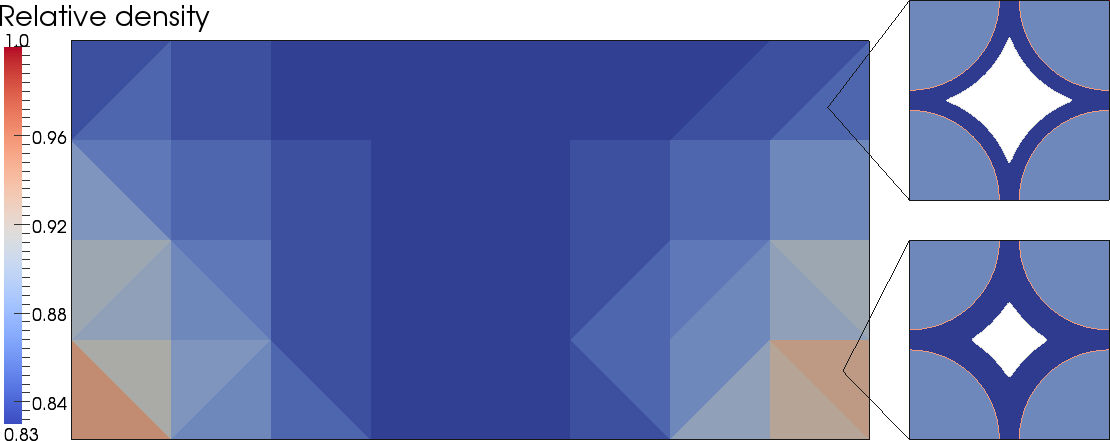
\includegraphics[width=\linewidth]{figures/macro_fe2_0000}
%  \caption{FE2}
%  \label{fig:final_dirichlet}
% \end{figure}

\begin{figure}[H]
 \centering
 \begin{tikzpicture}
  \node at (0,0) {
\includegraphics[scale=0.15]{figures/initial_rve}};
  \node at (4,2) {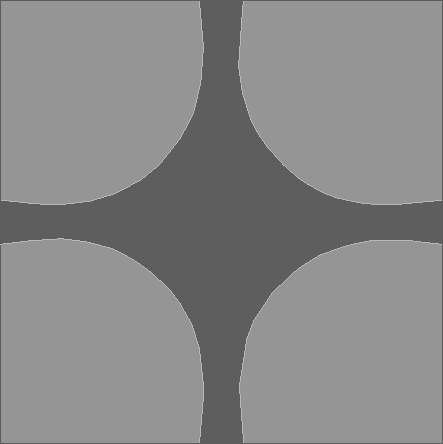
\includegraphics[scale=0.15]{figures/final_dirichlet}};
  \node at (4,-2) {
\includegraphics[scale=0.15]{figures/final_neumann}};
  \node at (0,1.5) {Initial};
  \node at (4,3.5) {Dirichlet};
  \node at (4,-0.5) {Neumann};
  \draw[-latex] (1.5,0.5) -- (2.5,1);
  \draw[-latex] (1.5,-0.5) -- (2.5,-1);
  \node at (8,2) {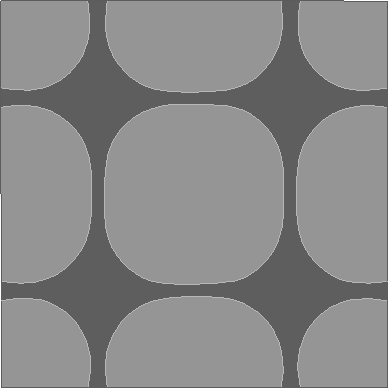
\includegraphics[scale=0.2]{figures/rve_dirichlet_2}};
  \node at (8,-2) {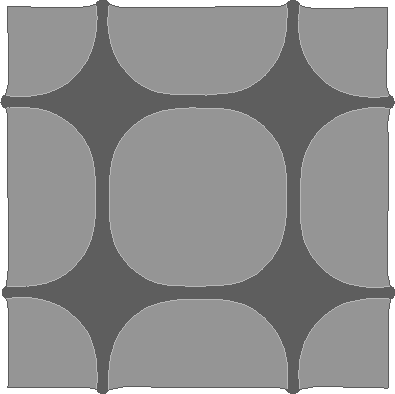
\includegraphics[scale=0.2]{figures/rve_neumann_2}};
 \end{tikzpicture}
 \caption{Initial and final state of 2D RVEs subject to free sintering}
 \label{fig:final_neumann}
\end{figure}

\begin{figure}[H]
 \centering
\begin{tikzpicture}
 \begin{axis}[
    width=0.8\linewidth,
    height=0.4\linewidth,
    ylabel={Relative density},xlabel={Time (scaled)},
    xmax=1, xmin=0, ymax=1.01, ymin=0.83,
    cycle list name=linestyles,
    yticklabel style={font=\tiny}, xticklabel style={font=\tiny},
%     scaled y ticks=manual:{}{\pgfmathparse{#1*100}}, % Scale for percentage
%     scaled x ticks=manual:{}{\pgfmathparse{#1*1000}}, % Scale for percentage
    legend style={draw=black,rounded corners=3pt,font=\footnotesize},
    legend pos=south east
    ]
  \addplot[blue ,densely dashed] table[y index=2] {figures/macro_3_dirichlet_x.out.matdata};
  \addlegendentry {Dirichlet 3$\times$3}
  \addplot[red  ,densely dashed] table[y index=2] {figures/macro_2_dirichlet_x.out.matdata};
  \addlegendentry {Dirichlet 2$\times$2}
  \addplot[black,densely dashed] table[y index=2] {figures/macro_1_dirichlet_x.out.matdata};
  \addlegendentry {Dirichlet 1$\times$1}

  \addplot[blue ] table[y index=2] {figures/macro_3_neumann_x.out.matdata};
  \addlegendentry {Neumann 3$\times$3}
  \addplot[red  ] table[y index=2] {figures/macro_2_neumann_x.out.matdata};
  \addlegendentry {Neumann 2$\times$2}
  \addplot[black] table[y index=2] {figures/macro_1_neumann_x.out.matdata};
  \addlegendentry {Neumann 1$\times$1}
 \end{axis}
\end{tikzpicture}
 \caption{Evolution of porosity with time for a 1$\times$1, 2$\times$2, and 3$\times$3  2D unit-cell subjected to zero macroscopic pressure, $\bar{p} = 0$.}
 \label{fig:porosity}
\end{figure}






\begin{figure}[H]
 \centering
 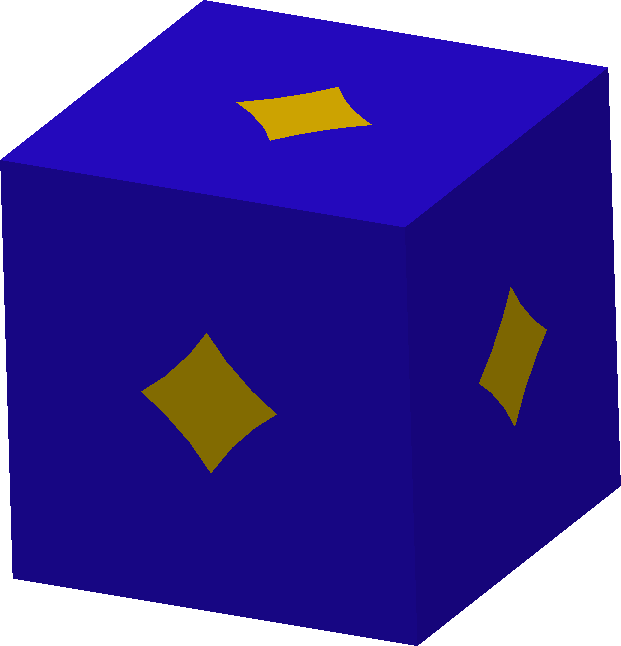
\includegraphics[height=0.3\linewidth]{figures/eightspheres}
 
\includegraphics[height=0.3\linewidth]{figures/eightspheres_cut}
 \caption{Initial state of 3D unit-cell with middle cross-section visible (right).}
 \label{fig:rve_3d}
\end{figure}


\begin{figure}[H]
 \centering
 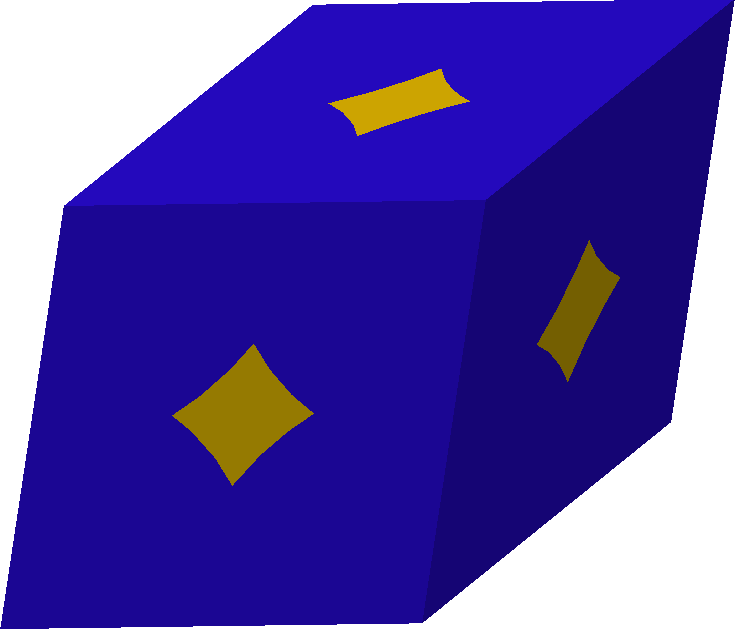
\includegraphics[width=0.3\linewidth]{figures/eightspheres_d_shear}
 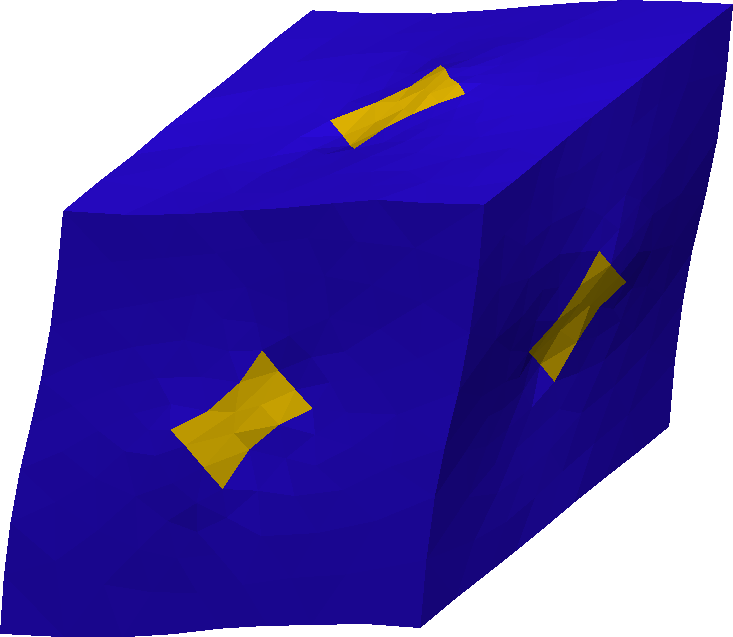
\includegraphics[width=0.3\linewidth]{figures/eightspheres_p_shear}
 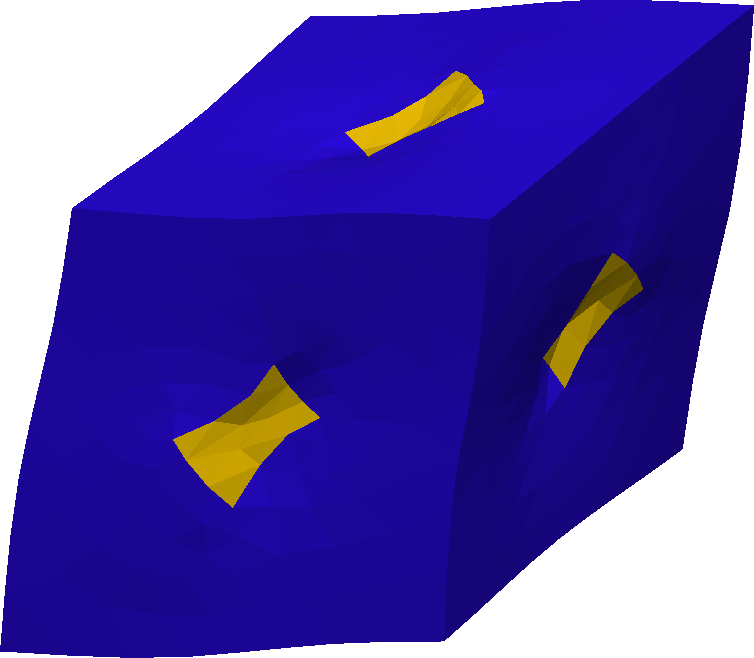
\includegraphics[width=0.3\linewidth]{figures/eightspheres_n_shear}
 \caption{3D unit-cell subject to pure shear. Boundary conditions are in order; Dirichlet, weakly periodic, and Neumann}
 \label{fig:rve_3d_deformed}
\end{figure}

\begin{table}[H]
 \centering

% # IST_DeviatoricStress, IST_Viscosity
% 6  0.000474658 0.00255358 -0.00302823  -0.000295588 -0.00137175   0.00186331 1 4.02824 % Dirichlet
% 6 -0.00144386  0.00113675  0.0013641    0.00308251   0.000218519 -0.00177107 1 3.44272 % Neumann
% 6 -0.00144378  0.000604311 0.000839466 -0.00175045  -7.27793e-05  0.00321311 1 0.440223 % Periodic


 %\includegraphics[width=0.4\linewidth]{figures/eightspheres_d_final}
 %\includegraphics[width=0.4\linewidth]{figures/eightspheres_n_final}
 \caption{Homogenized values from the 3D unit-cell subject to free sintering at time zero}
 \label{tab:rve_3d_homog}
\end{table}


% \begin{figure}[H]
%  \centering
% PLACEHOLDER
%  %\includegraphics[width=0.4\linewidth]{figures/eightspheres_d_final}
%  %\includegraphics[width=0.4\linewidth]{figures/eightspheres_n_final}
%  \caption{3D RVE of Dirichlet (left) and Neumann (right) type subject to free sintering}
%  \label{fig:rve_3d_final}
% \end{figure}

In \cref{fig:rve_3d_deformed} displacements of an RVE can be seen exaggerated as to show the slight differences from the weakly periodic and Neumann boundary condition.
Homogenized macroscopic viscosity, $\bar{\mu}$, can be computed by the minimization
\begin{align}
 \min \frac12 \sum_{ijkl} (\bar{\tf E} - 2 \bar{\mu} \tf I_\dev)_{ijkl}^2 \implies \bar{\mu} = \frac12 \frac{\sum_{ijkl}(\tf I_\dev)_{ijkl}(\bar{\tf E})_{ijkl}}{\sum_{ijkl} (\tf I_\dev)_{ijkl}^2}
\end{align}
where $\tf I_\dev$ is the deviatoric fourth order identity tensor such that the isotropic part of $\bar{\tf E}$ can be expressed as $\bar{\tf E}_{\mathrm{iso}} = 2 \bar{\mu} \tf I_\dev$ in standard fashion.
For the RVE in \cref{fig:rve_3d}, one can find for each respective boundary condition; Dirichlet $\bar{\mu}^\Dirichlet = 4.024 \mu_\binder$, periodic $\bar{\mu}^\Periodic = 3.675\mu_\binder$, Neumann $\bar{\mu}^\Neumann = 3.433\mu_\binder$.
As expected, the Neumann and Dirichlet boundary condition does act as bounds, i.e.\ $\bar{\mu}_\particle \geq \bar{\mu}^\Dirichlet \geq \bar{\mu}^\Periodic \geq \bar{\mu}^\Neumann$.
%   3.67483  % Periodic
%   4.02441  % Dirichlet
%   3.43327  % Neumann


The RVE is capable of capturing anisotropic effects, which is something that most macroscopic material models are unable to capture due to only considering the porosity and not the shape.




\section{Conclusions and outlook}

In this paper, we have shown a variationally consistent homogenization procedure that allows for internal pores with surface tension, in a medium that may be incompressible.
When all microconstituents are intrinsically incompressible, we may still obtain macroscopic deformation if pores are present.
The case of sintering, where pores, driven by surface tension, are allowed to completely vanish, can now be captured in this homogenization scheme. 

By carefully choosing the prolongation of the macroscopic fields onto $\ta v^\macro$ and $p^\macro$, we have shown that one obtains the same simple macroscopic formulation as in \cite{ohman_variationally_2014}, even when taking into account both porosity and surface tension.
Furthermore, by isolating the post-processing procedure of the macroscopic variables $\bar{\ts\sigma}_\dev$ and $\bar{e}$ to the RVE-boundary, $\Gamma_\rve$, an identical procedure to that of \cite{ohman_variationally_2014} where pores where not present is obtained.
Worth pointing out is that deriving the macroscale format and the Dirichlet boundary condition by VCH yields identical results that in \cite{ohman_computational_2013}, where only the velocity field was homogenized.


We have also shown that surface tension on micropores can actually have contributions to $\bar{\ts\sigma}_\dev$, which is not captured in traditional macroscale material models of the ``sintering-stress'' which is usually defined as a macroscopic pressure resulting from surface tension on micro pores.
This can play an important role in sintering, where the pores in the metal powder that can be distorted from the compaction process.
This effect is captured naturally in an RVE which can take into account anisotropic effects of pores.


In order to derive the weakly periodic and Neumann boundary conditions, we have been required to consider only RVEs that have no pores on the boundary as we need to apply a traction over the entire RVE-boundary.
This puts an ultimate limitation to the realism of the microstructure when using the Neumann and Weakly periodic boundary condition.


The large deformations of the RVEs requires remeshing which are particularly challenging for free surface flow in 3D.
Alternatives to remeshing, such as \cite{pino_munoz_direct_2013} which uses level-sets to describe the geometry of multiple randomized particles can be used to alleviate the need for complicated remeshing strategies.


\printbibliography

\end{document}